\chapter{Results}
\section{Implementation of Randomness in the Logistic Map}
We explored how the random logistic map changes in terms of its
bifurcation diagram and Lyapunov exponents, and also the distribution
of period $p$ orbits in terms of a set of histograms. The variance of
$\xi(x)$ was simulated for two values: the maximum value and
half of the maximum value from~(\ref{sigma}).

An unexpected result of the simulations is the presence of the stable
periodic orbits in the right side of the bifurcation diagram. These
stable orbits appear for both the case where the variance $\sigma$ of
$\xi(x)$ from~(\ref{sigma}) is chosen to be the maximal value and the
case where we choose half of the maximal
value. Figure~\ref{fig:rlogbif} and Figure~\ref{fig:rlogbif_zoom}
correspond to choosing $\sigma$ to be the maximum, and
Figure~\ref{fig:rlogbif_hs} and Figure~\ref{fig:rloglyap2_hs} to half
of the maximum. Specifically, this stable region occurs between $r\in [3,4]$, and is most dominantly featured for the bifurcation
diagrams with $L=0.1$. Figure~\ref{fig:rlogbif_zoom} zooms in on the
range $r \in [3,4]$ to show the newly stabilized region more clearly. In the
deterministic case (Figure~\ref{fig:bif}), this region was previously
unstable. 

Examining the Lyapunov exponent of the random logistic
map for the case where $\sigma$ is large gives some insight on whether
the map is possibly chaotic. The exponent of the deterministic map is
on the top left of Figure~\ref{fig:rloglyap2}, and we see there is a
point in $r$ where stable behavior transitions to chaotic behavior (just under $r=3.6$). In the randomized case, the
delimination is unclear. However one feature of the deterministic
diagram seems to be preserved, and that is the negative spike around
$r=3.8$, which corresponds to an island of stability in the
deterministic map.

\begin{figure}[H]\linespread{1}
\caption[Bifurcation diagram of the random logistic map, $\sigma=\sigma_{max}$]{Bifurcation diagram of the random
logistic map, where $r \in [0,4]$, $\Delta r = 0.002$, $N=100$, the
number of initial conditions tested is $N_{x_0}$, $L\in
\{0.1,0.2,0.4,0.6,0.8,0.9\}$, and $\sigma$ is chosen to be the maximal
value in the interval from~(\ref{sigma}). Plots are read left to right, and top to
bottom. Number of simulations is 1.8 million. The colorbar shows the color for each period. Orbits up to period 256 were checked.}\label{fig:rlogbif}
	\begin{center}
		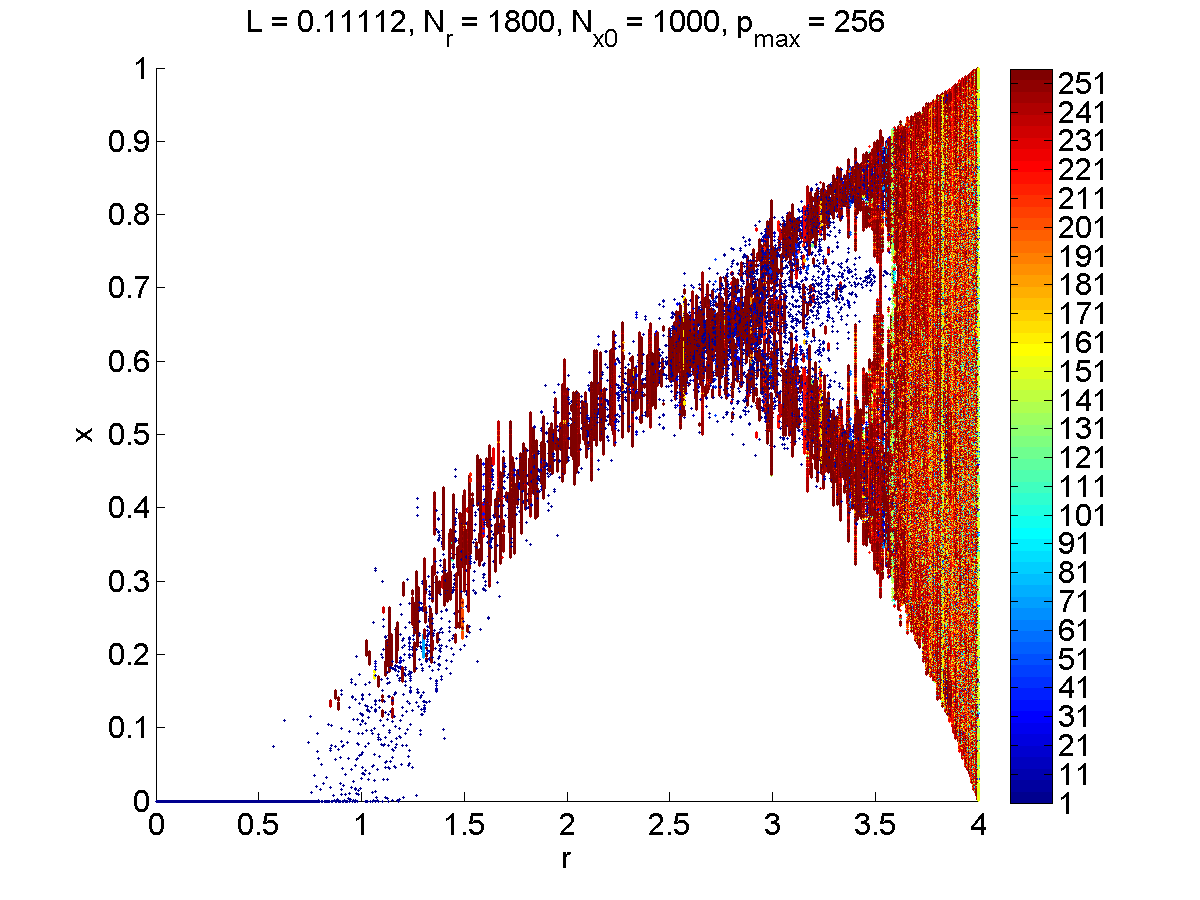
\includegraphics[width=.5\textwidth]{figs/rlog_bif_L_01.png}\hfill
		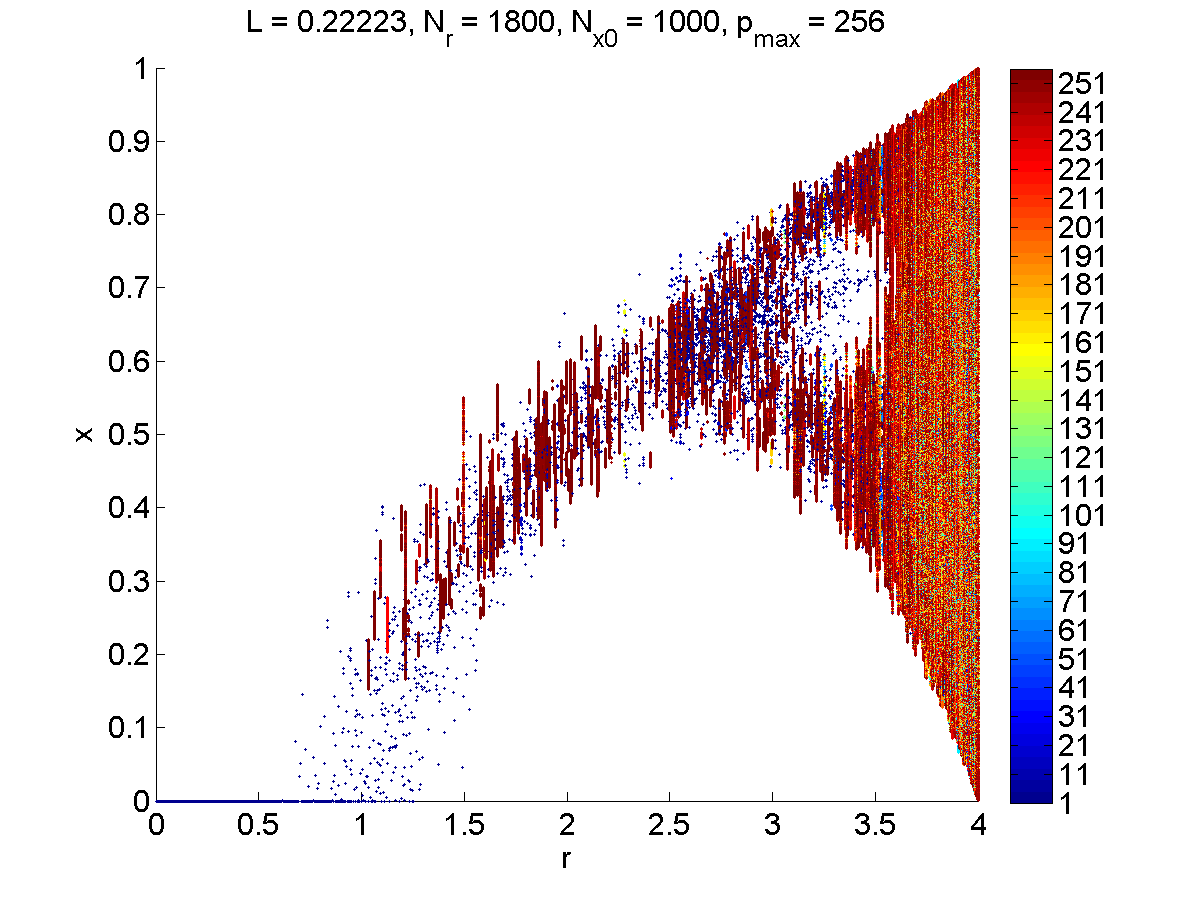
\includegraphics[width=.5\textwidth]{figs/rlog_bif_L_02.png}\\
		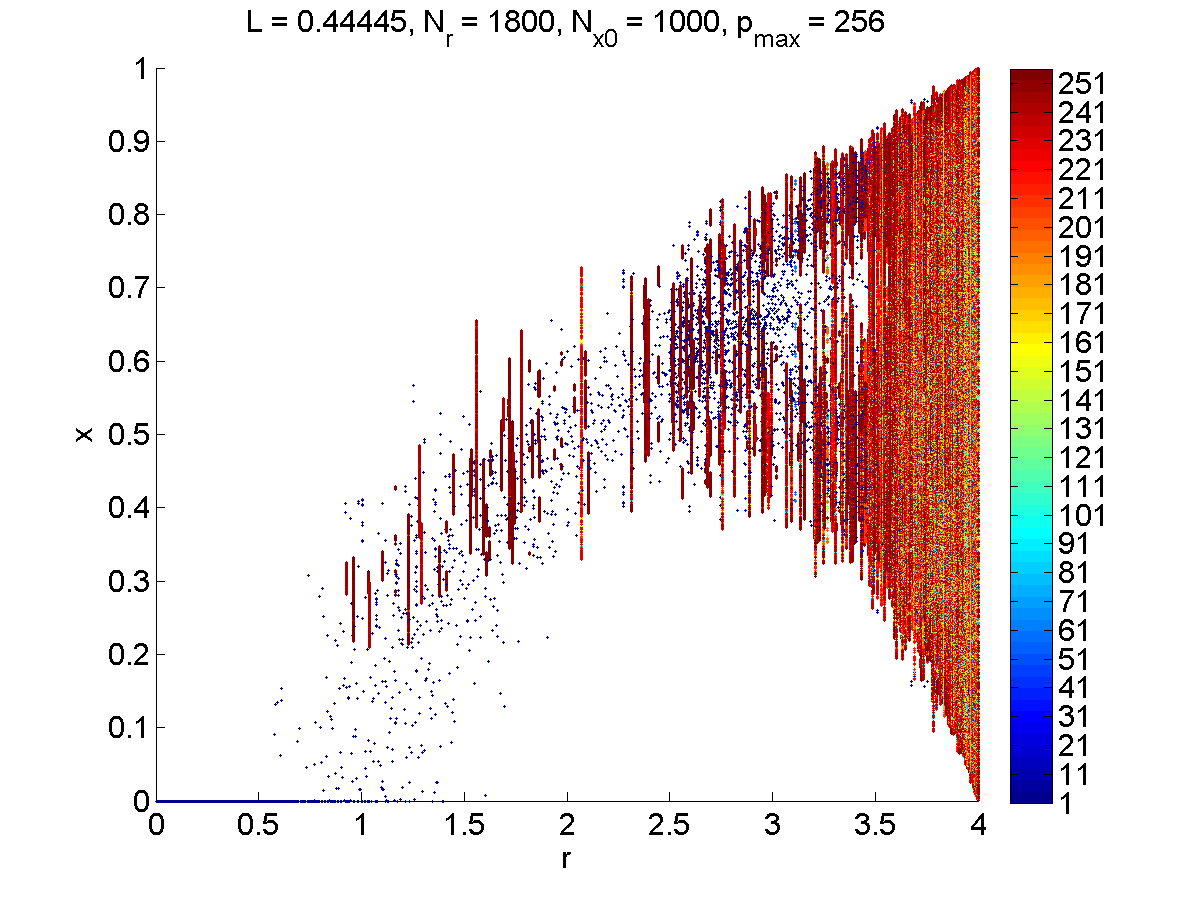
\includegraphics[width=.5\textwidth]{figs/rlog_bif_L_04.png}\hfill
		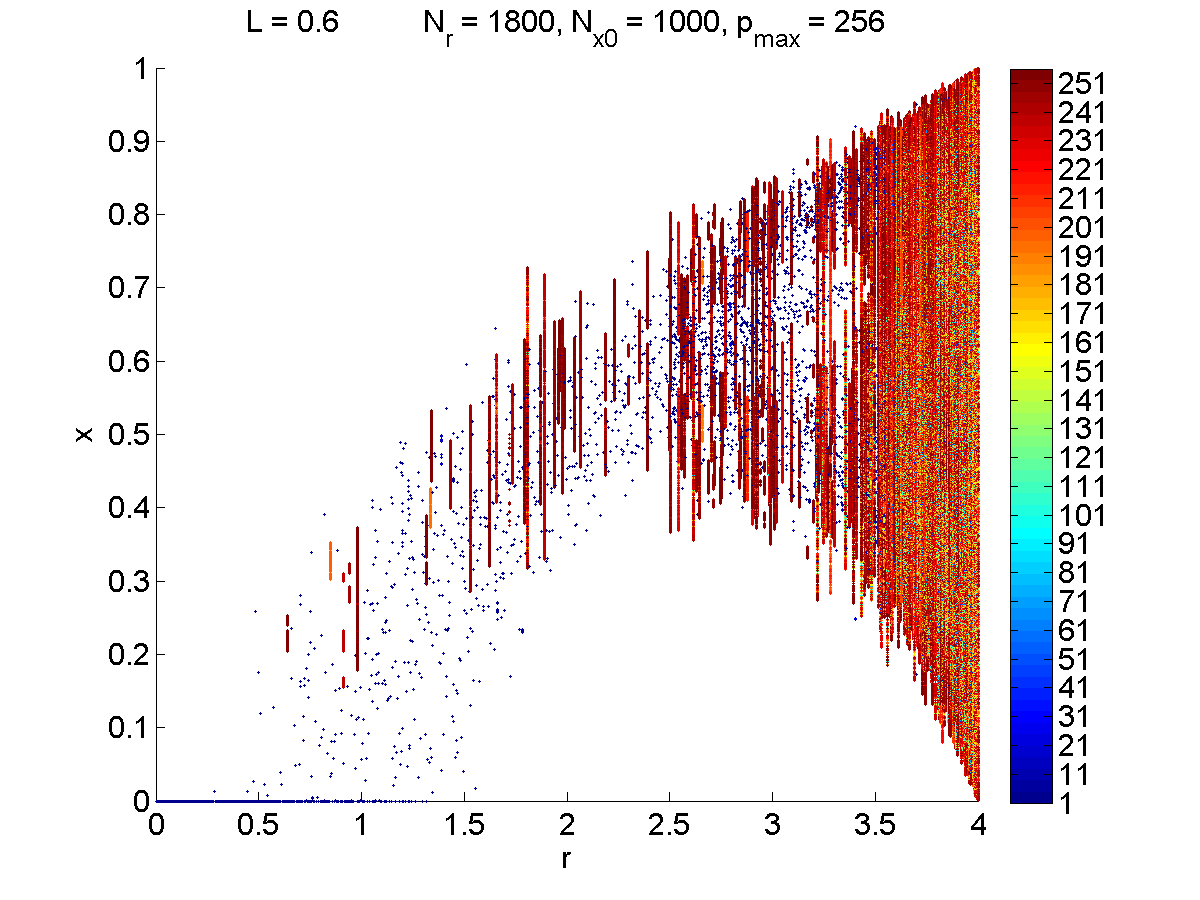
\includegraphics[width=.5\textwidth]{figs/rlog_bif_L_06.png}\\
		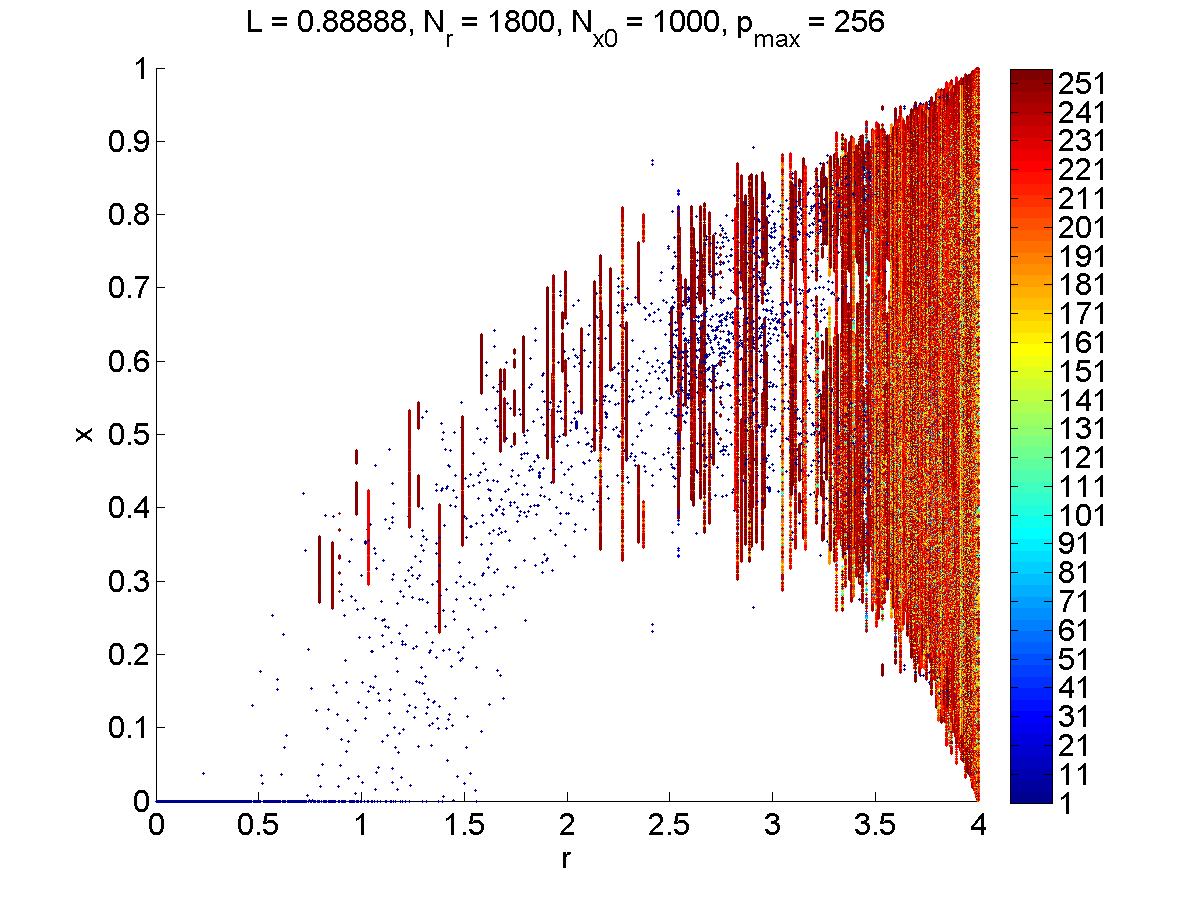
\includegraphics[width=.5\textwidth]{figs/rlog_bif_L_08.png}\hfill
		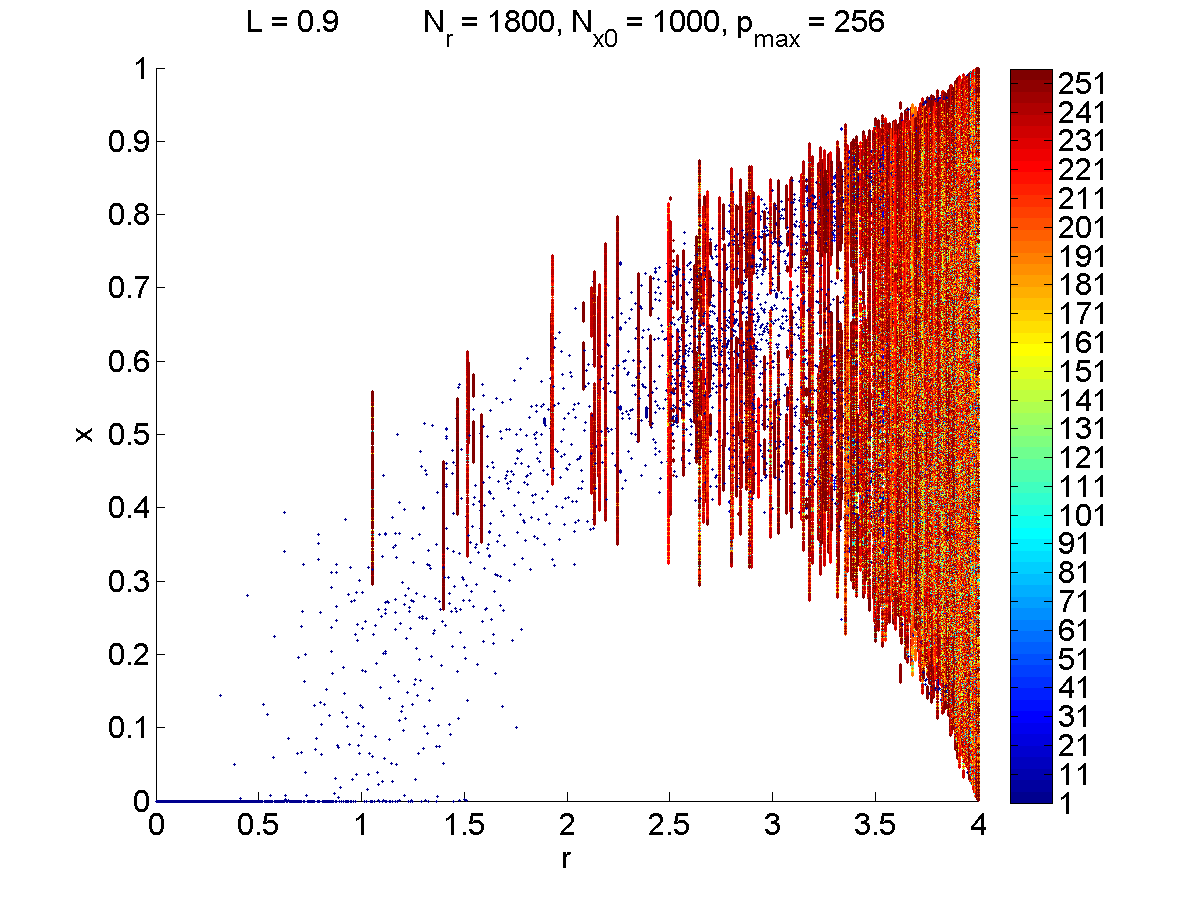
\includegraphics[width=.5\textwidth]{figs/rlog_bif_L_09.png}\\
	\end{center}
\end{figure}

\begin{figure}[H]\linespread{1}
\caption[Bifurcation diagram of the random logistic map, $\sigma=\sigma_{max}$, zoomed
in]{A zoomed in view of Figure~\ref{fig:rlogbif}, where $r \in
  [3,4]$, $\Delta r = 0.001$, $N=100$, the number of initial
  conditions tested is $N_{x_0}$, $L\in \{0.1,0.2,0.4,0.6,0.8,0.9\}$,
  and $\sigma$ is chosen to be the maximal
value in the interval from~(\ref{sigma}). Plots are read left to right, and top to
bottom. Number of simulations is 1.8 million. The colorbar shows the color for each period. Orbits up to period 256 were checked.}\label{fig:rlogbif_zoom}
	\begin{center}
		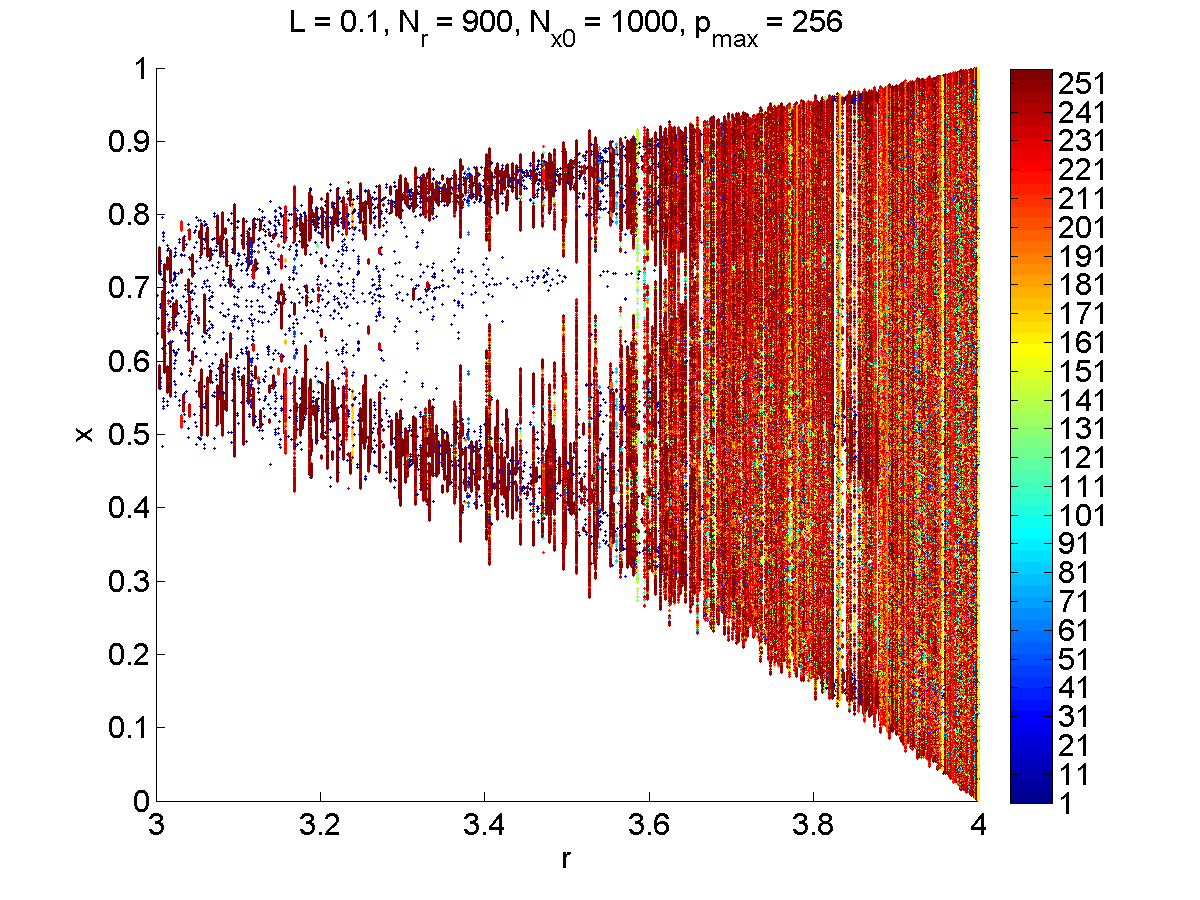
\includegraphics[width=.5\textwidth]{figs/rlog_bif_zoom_L_01.png}\hfill
		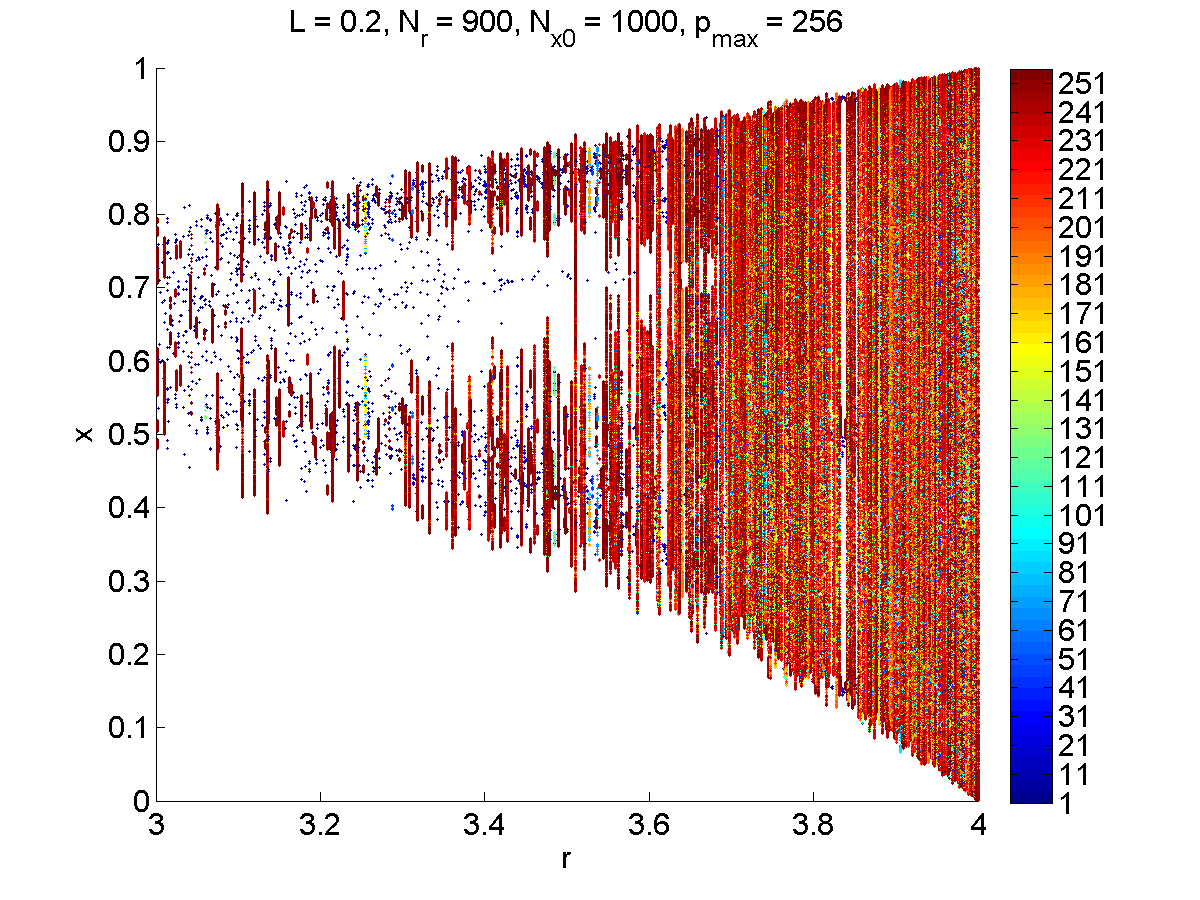
\includegraphics[width=.5\textwidth]{figs/rlog_bif_zoom_L_02.png}\\
		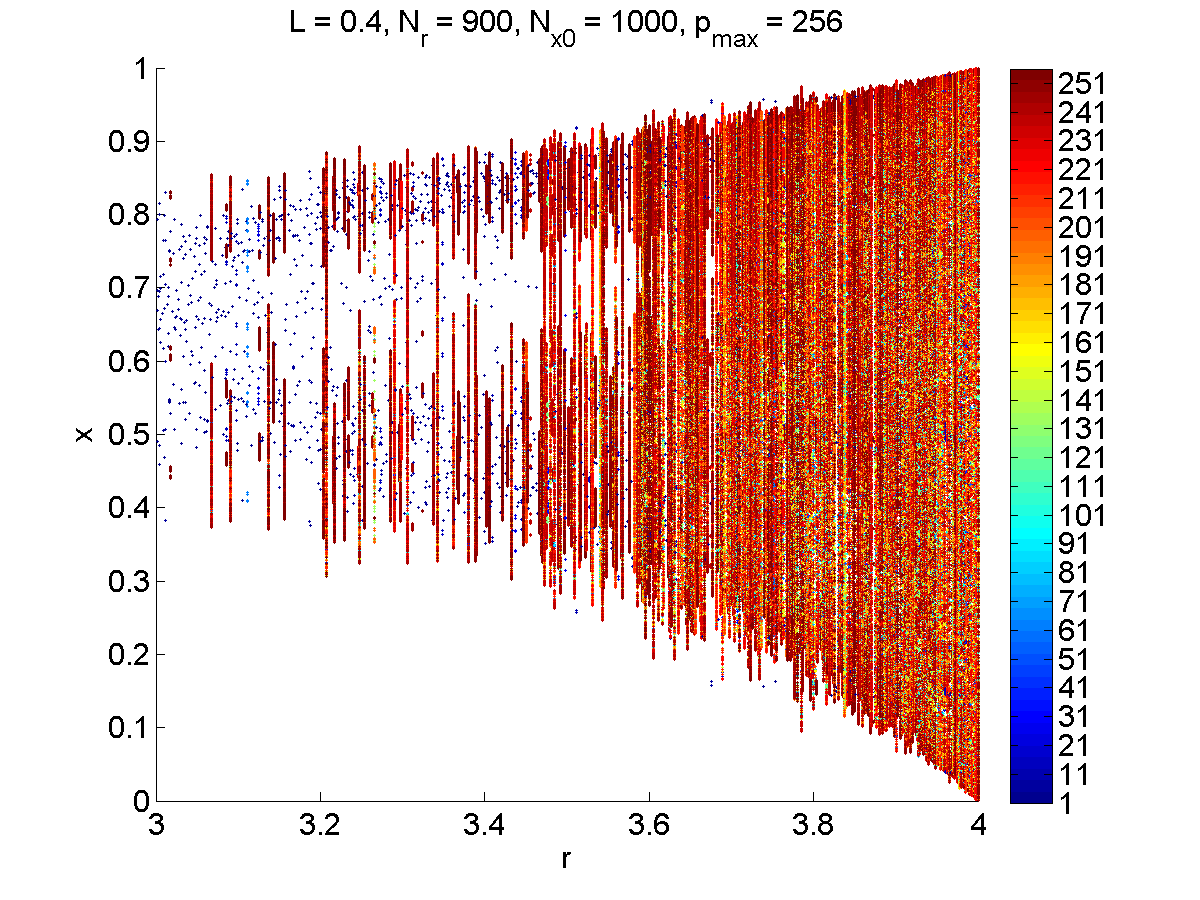
\includegraphics[width=.5\textwidth]{figs/rlog_bif_zoom_L_04.png}\hfill
		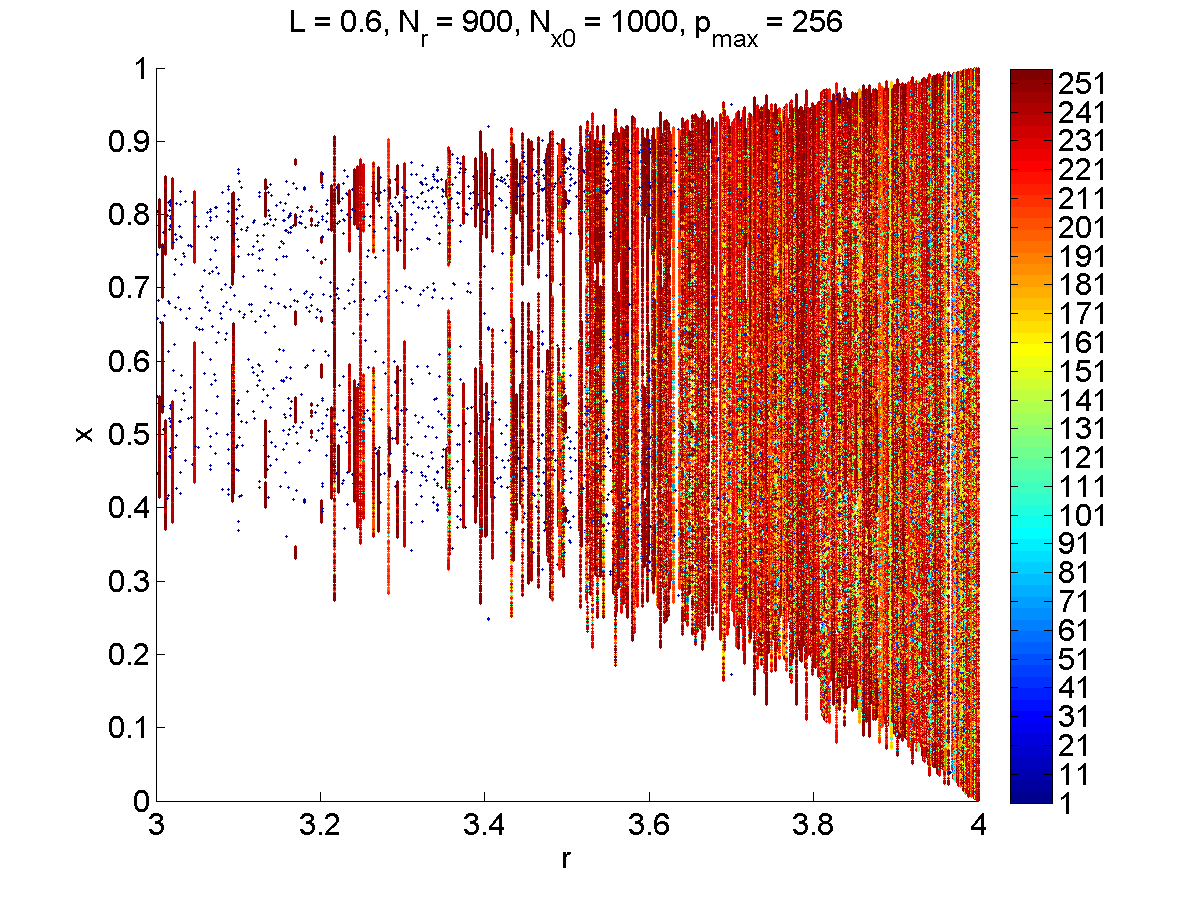
\includegraphics[width=.5\textwidth]{figs/rlog_bif_zoom_L_06.png}\\
		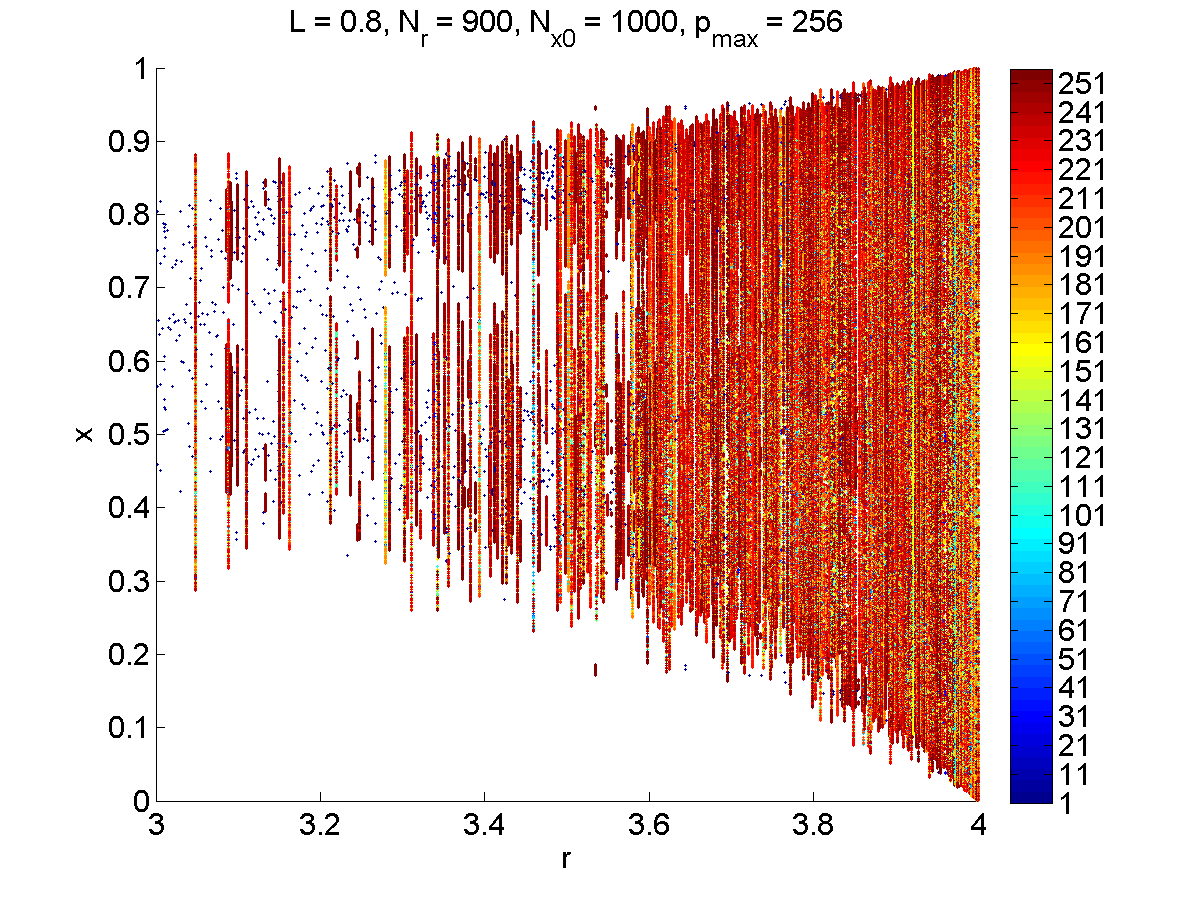
\includegraphics[width=.5\textwidth]{figs/rlog_bif_zoom_L_08.png}\hfill
		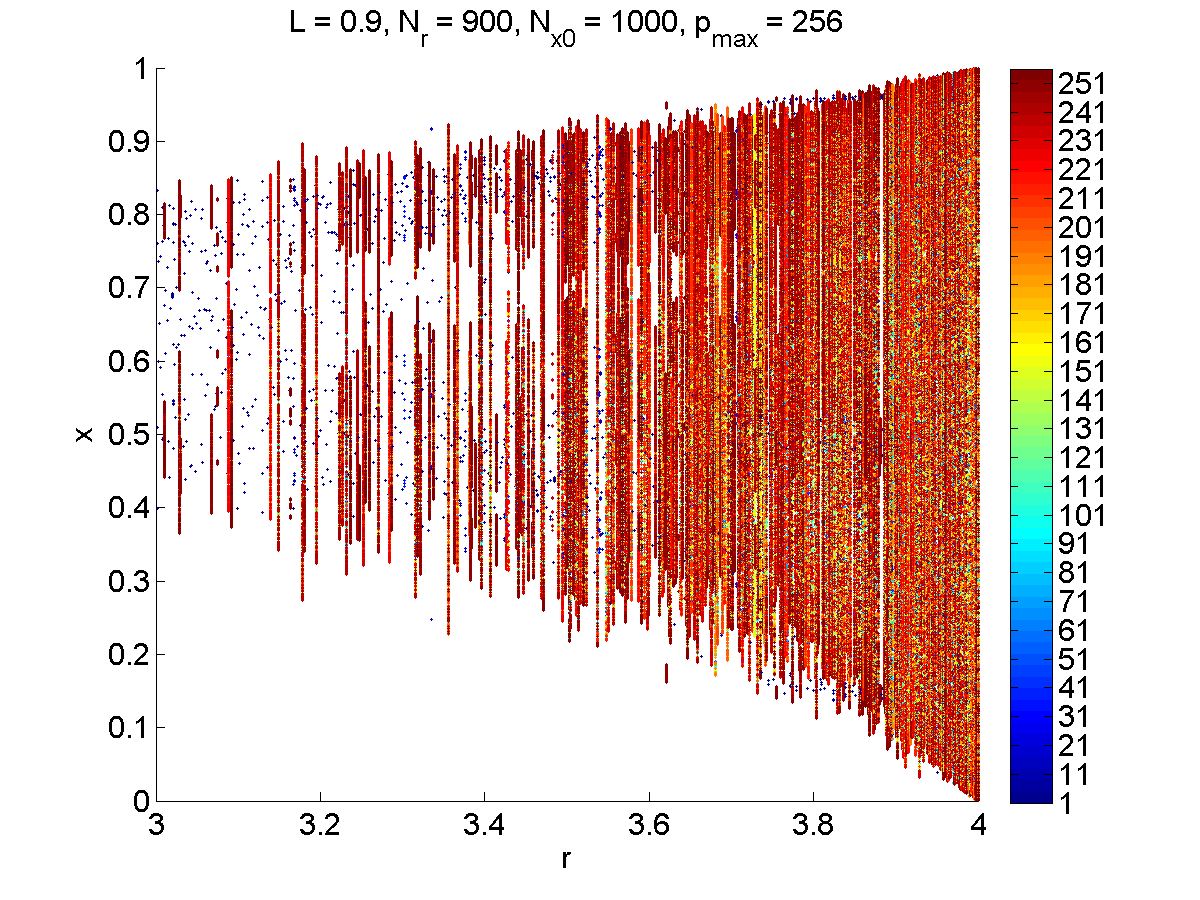
\includegraphics[width=.5\textwidth]{figs/rlog_bif_zoom_L_09.png}\\
	\end{center}
\end{figure}

\begin{figure}[!h]
\caption[Lyapunov exponent in the random logistic map compared to the
deterministic map, $\sigma=\sigma_{max}$]{The Lyapunov exponent for the deterministic
  logistic map (top left) is compared
  to the Lyapunov exponent of the random logistic map for $L \in
  \{0.05,0.1,0.5,0.7,0.9\}$, where $x_0=0.7$ for $r \in [3,4]$, and
  $\sigma$ is chosen to be the maximal value in the interval
  from~(\ref{sigma}). The number of exponents computed was $N_\lambda=10,000$. Plots are read left to right, and top to bottom. }\label{fig:rloglyap2}
\centering
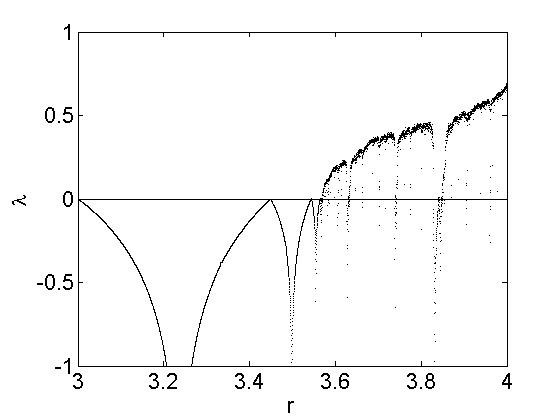
\includegraphics[width=.5\textwidth]{figs/det_log_lyap.png}\hfill
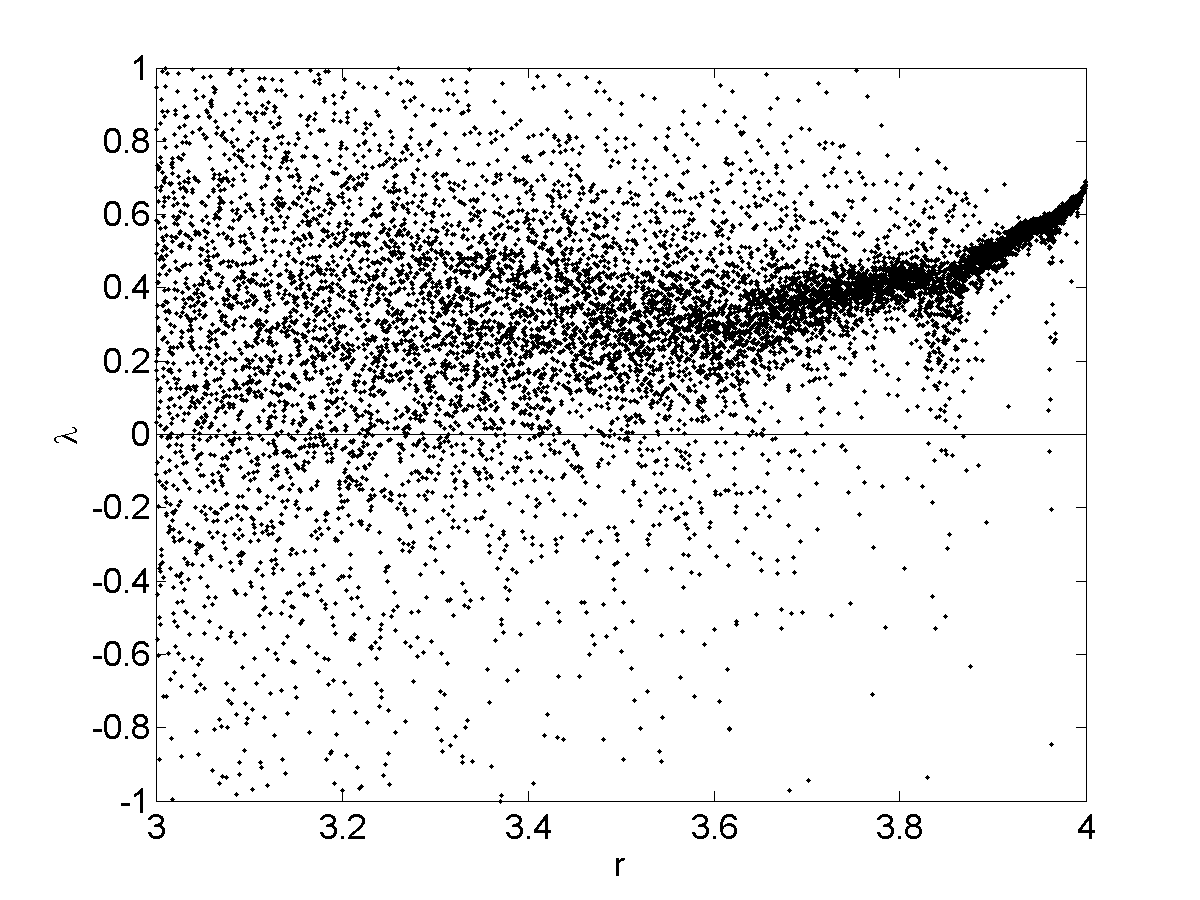
\includegraphics[width=.5\textwidth]{figs/rlog_lyap_L_005.png}\\
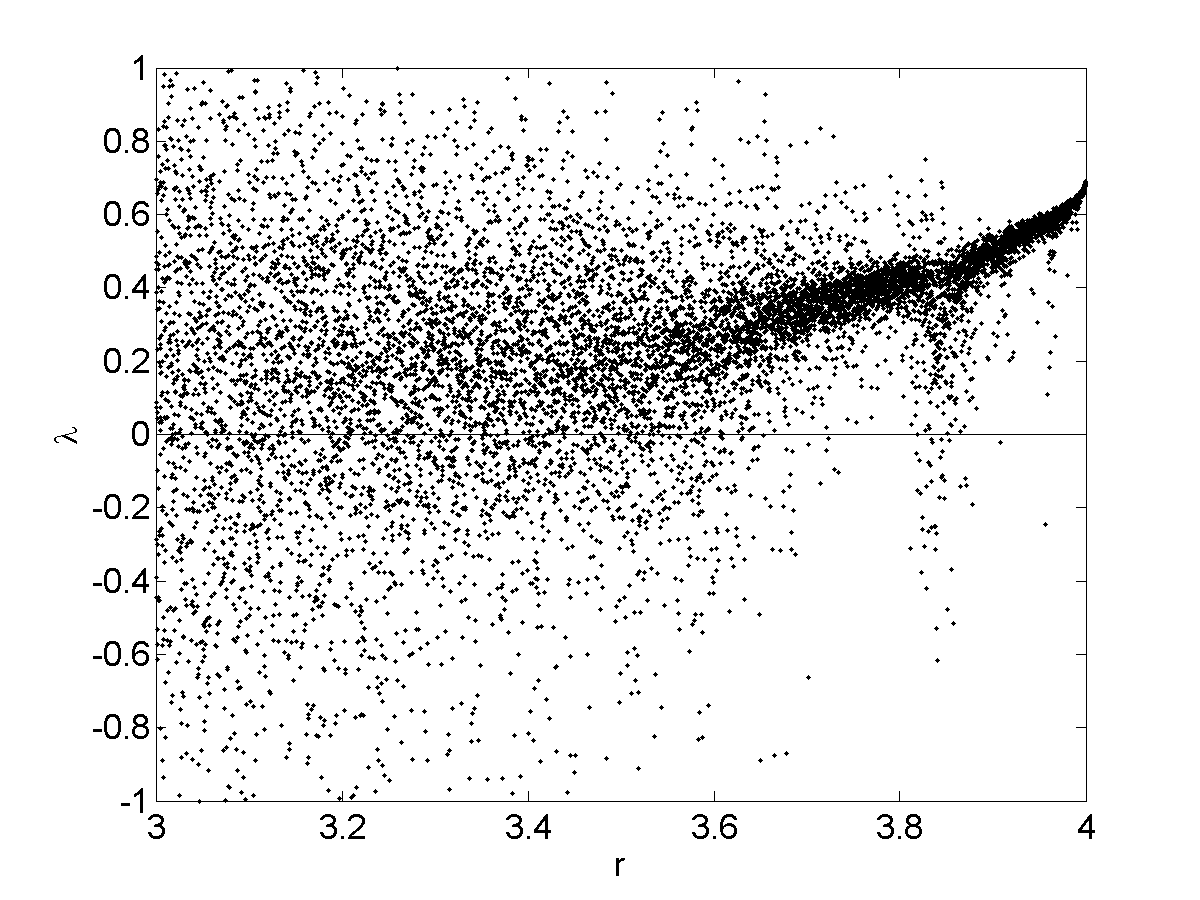
\includegraphics[width=.5\textwidth]{figs/rlog_lyap_L_01.png}\hfill
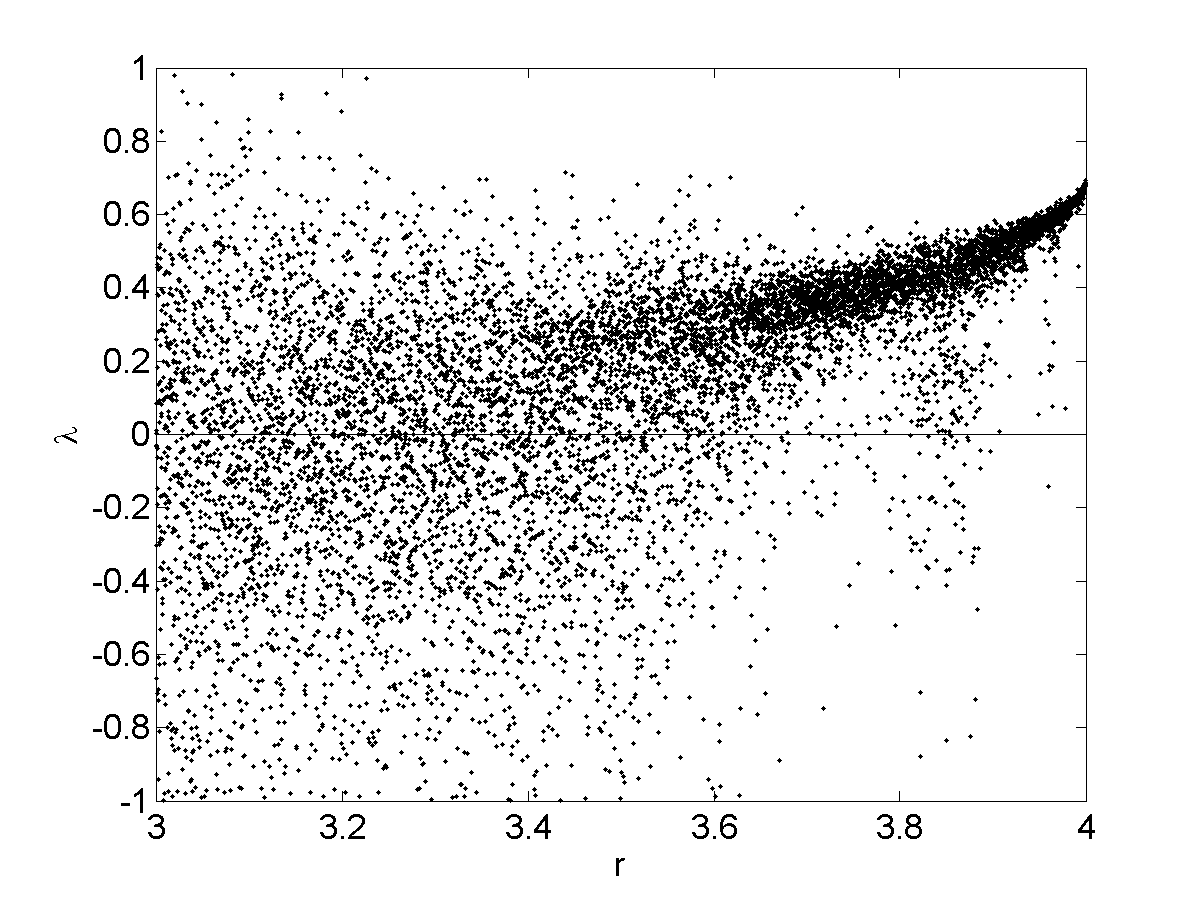
\includegraphics[width=.5\textwidth]{figs/rlog_lyap_L_05.png}\\
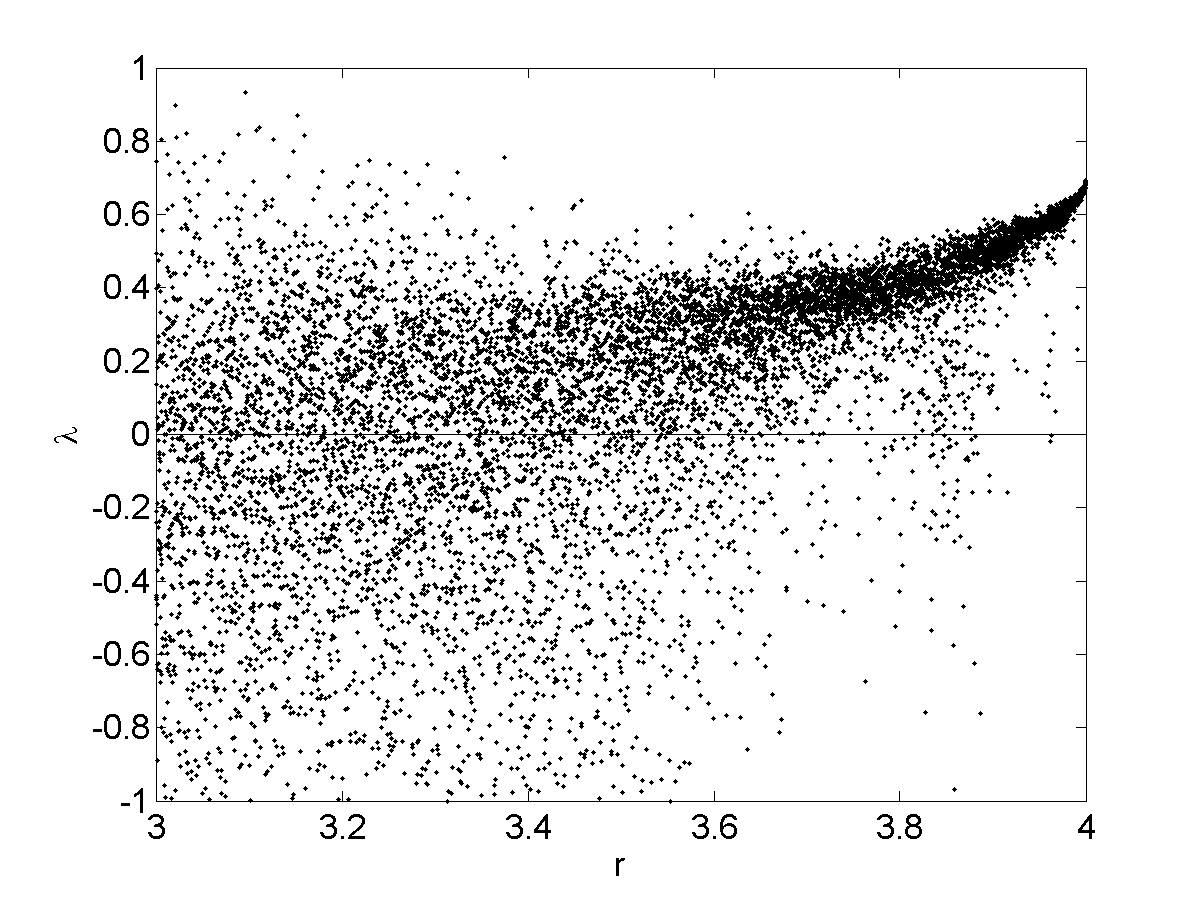
\includegraphics[width=.5\textwidth]{figs/rlog_lyap_L_07.png}\hfill
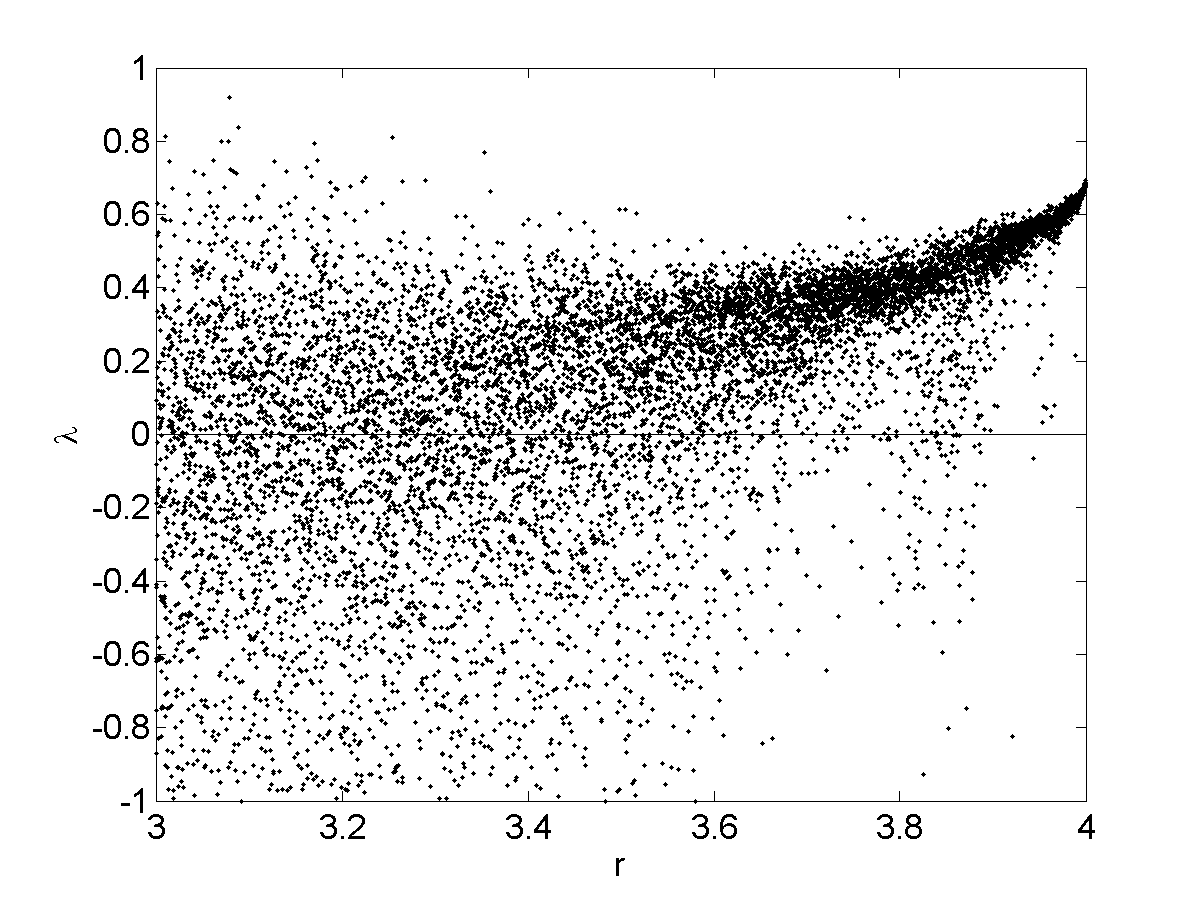
\includegraphics[width=.5\textwidth]{figs/rlog_lyap_L_09.png}\\
\end{figure}

A histogram describing the average fraction of observed period $p$
orbits is shown in Figure~\ref{fig:rloghist}. The histogram implies
that the most commonly observed stable orbit is period 2, and the
distribution of periodic orbits may follow the exponential
distribution. The distribution of period for any give $(r,L)$ pair
offers insight on the type of orbits that the random process solicits.

\begin{figure}[H]\linespread{1}
\caption[Average number of period $p$ orbits for the random logistic
map, $\sigma=\sigma_{max}$]{Average number of period $p$ orbits for the random logistic
map, where $r =3.2$,$L=0.1$,$N=100$, and $\sigma = 0.0061$. Results from 2000
simulations of these parameters are plotted. The error bars indicate
the standard error of the calculation of the mean for 2000 samples.}\label{fig:rloghist}
	\begin{center}
          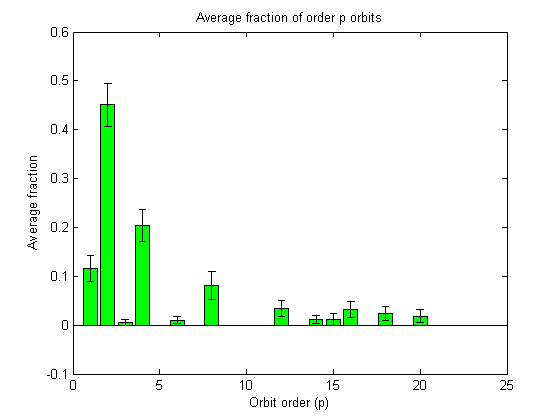
\includegraphics[scale=0.65]{figs/rlog_hist_r32_L01.png}
	\end{center}
\end{figure}

Figure~\ref{fig:rlogbif_hs} and Figure~\ref{fig:rloglyap2_hs}
demonstrate results from simulating the random logistic map where the
variance $\sigma$ of $\xi(x)$ is chosen to be half of the maximal
value from~(\ref{sigma}). Not surprisingly, the stable low period
orbits for $r \in [3,4]$ endure even
when the noise is restricted. Further, it appears the density of
stable orbits for $r<3$ diminishes as $L$ is increased. Additionally,
there are fewer stable high period orbits when $\sigma$ is small.

The positive Lyapunov exponents of the randomized logistic
map for the case where $\sigma$ is small in
Figure~\ref{fig:rloglyap2_hs} implies that even a halved standard
deviation will incur chaotic behavior. The negative spike around
$r=3.8$, which corresponds to an island of stability in the
deterministic map, is more prominent when $\sigma$ is small than when large. Between
Figure~\ref{fig:rloglyap2} and Figure~\ref{fig:rloglyap2_hs}, it
appears that decreasing $\sigma$ causes the plot of Lyapunov exponents
of the random map to fall more in line with the plot for the
deterministic map. There are fewer positive exponents in
Figure~\ref{fig:rloglyap2_hs} than in Figure~\ref{fig:rloglyap2}, and
remnants of other islands of stability from the deterministic map
appear in the plots of the random map (e.g. $r \approx 3.95$).

\begin{figure}[H]\linespread{1}
\caption[Bifurcation diagram of the random logistic map, $\sigma=\frac{1}{2}\sigma_{max}$]{Bifurcation diagram of the random
logistic map, where $r \in [0,4]$, $\Delta r = 0.002$, $N=100$, the
number of initial conditions tested is $N_{x_0}$, $L\in
\{0.1,0.2,0.4,0.6,0.8,0.9\}$, and $\sigma$ is chosen to be half of the maximal
value in the interval from~(\ref{sigma}). Plots are read left to right, and top to
bottom. Number of simulations is 1.8 million. The colorbar shows the color for each period. Orbits up to period 256 were checked.}\label{fig:rlogbif_hs}
	\begin{center}
		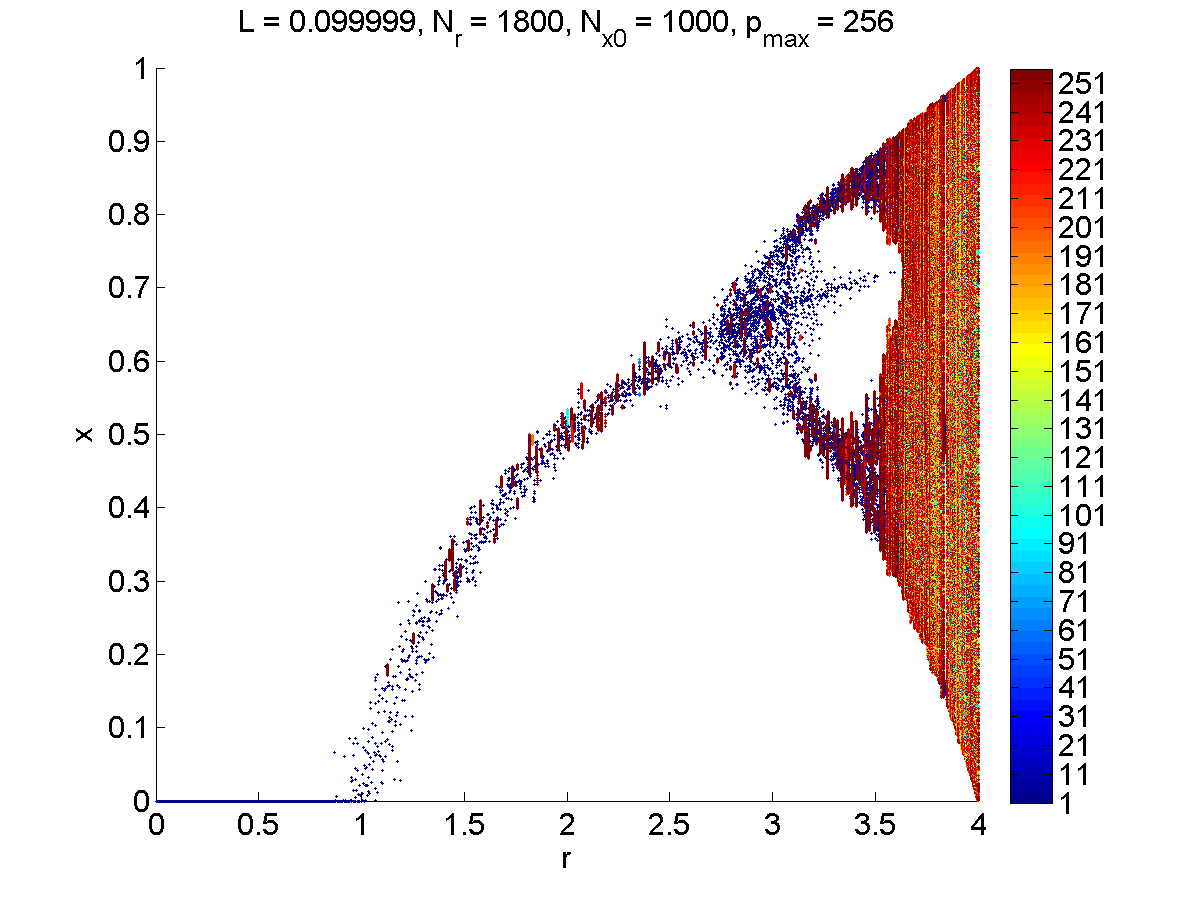
\includegraphics[width=.5\textwidth]{figs/rlog_bif_halfs_L_01.png}\hfill
		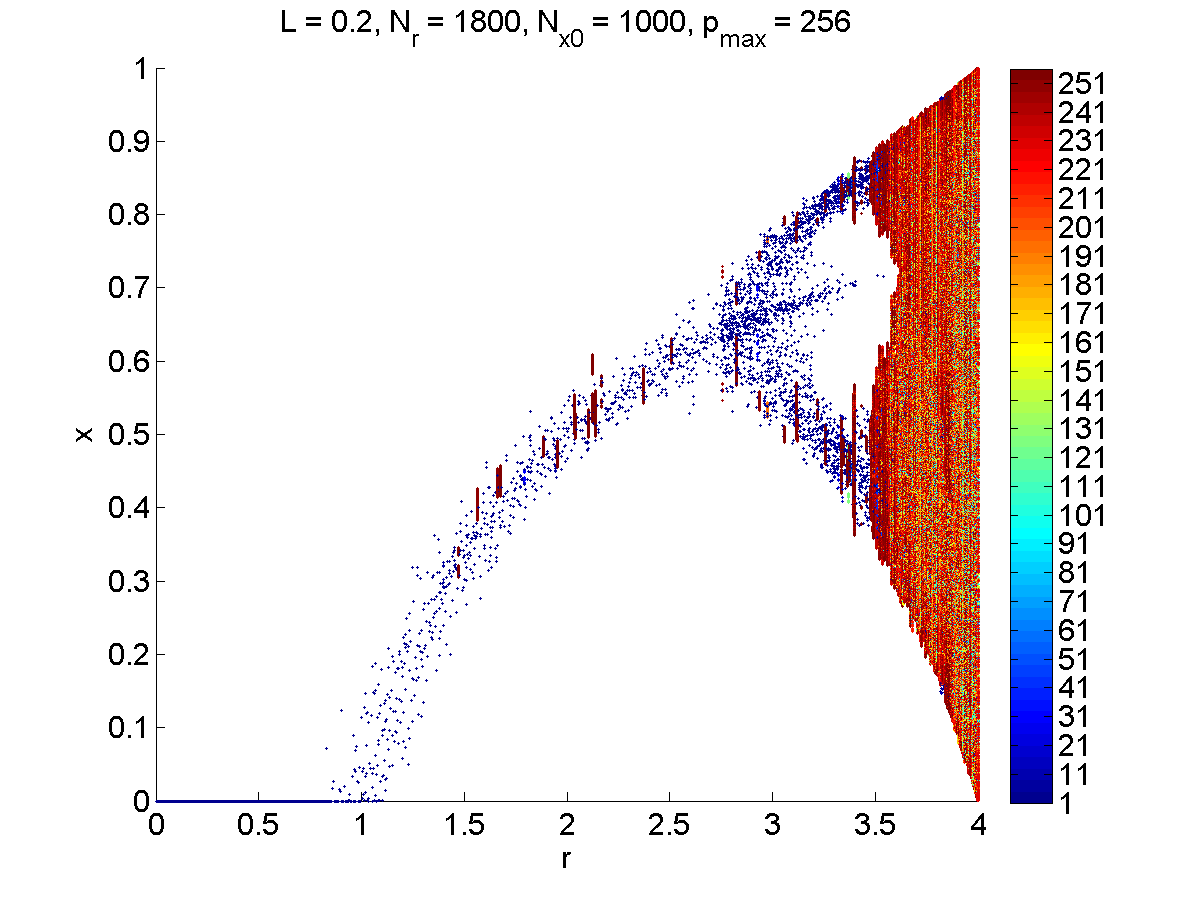
\includegraphics[width=.5\textwidth]{figs/rlog_bif_halfs_L_02.png}\\
		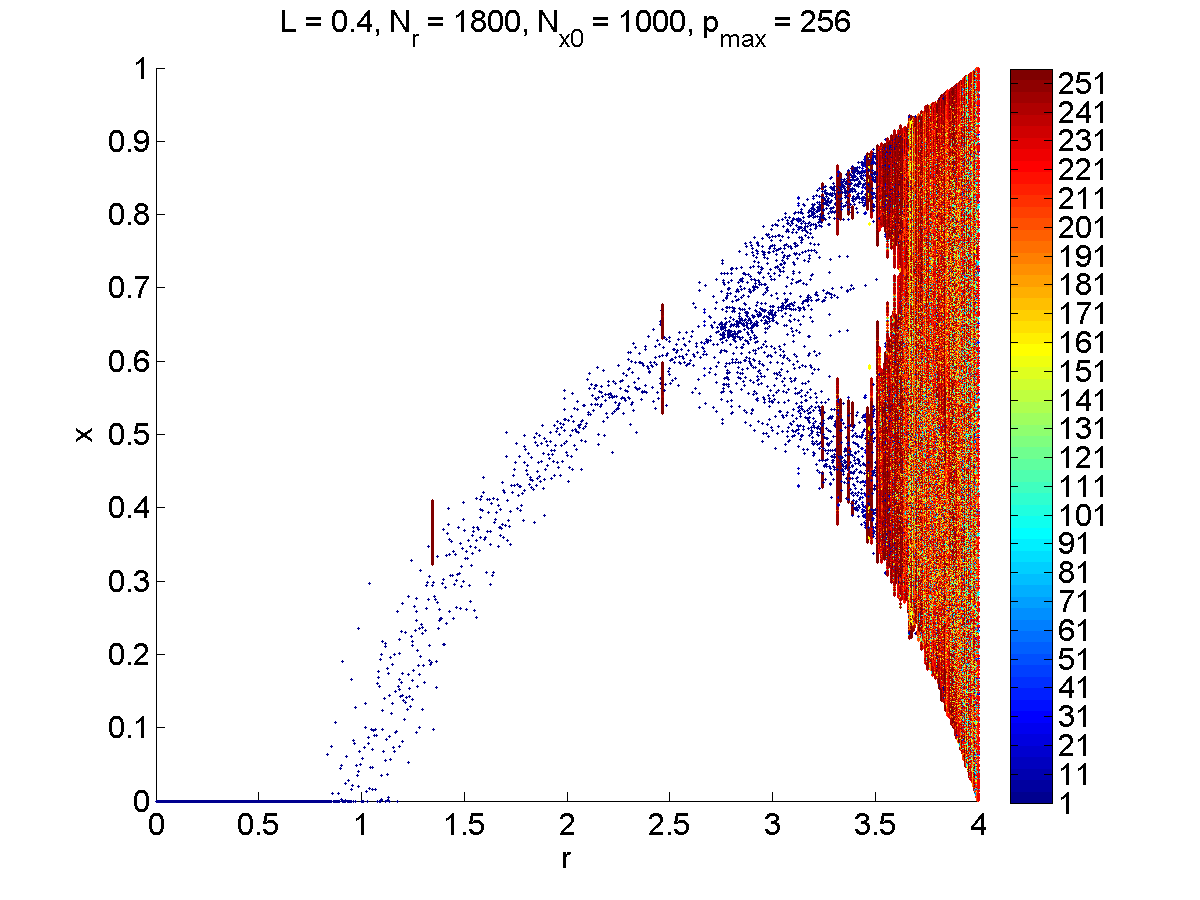
\includegraphics[width=.5\textwidth]{figs/rlog_bif_halfs_L_04.png}\hfill
		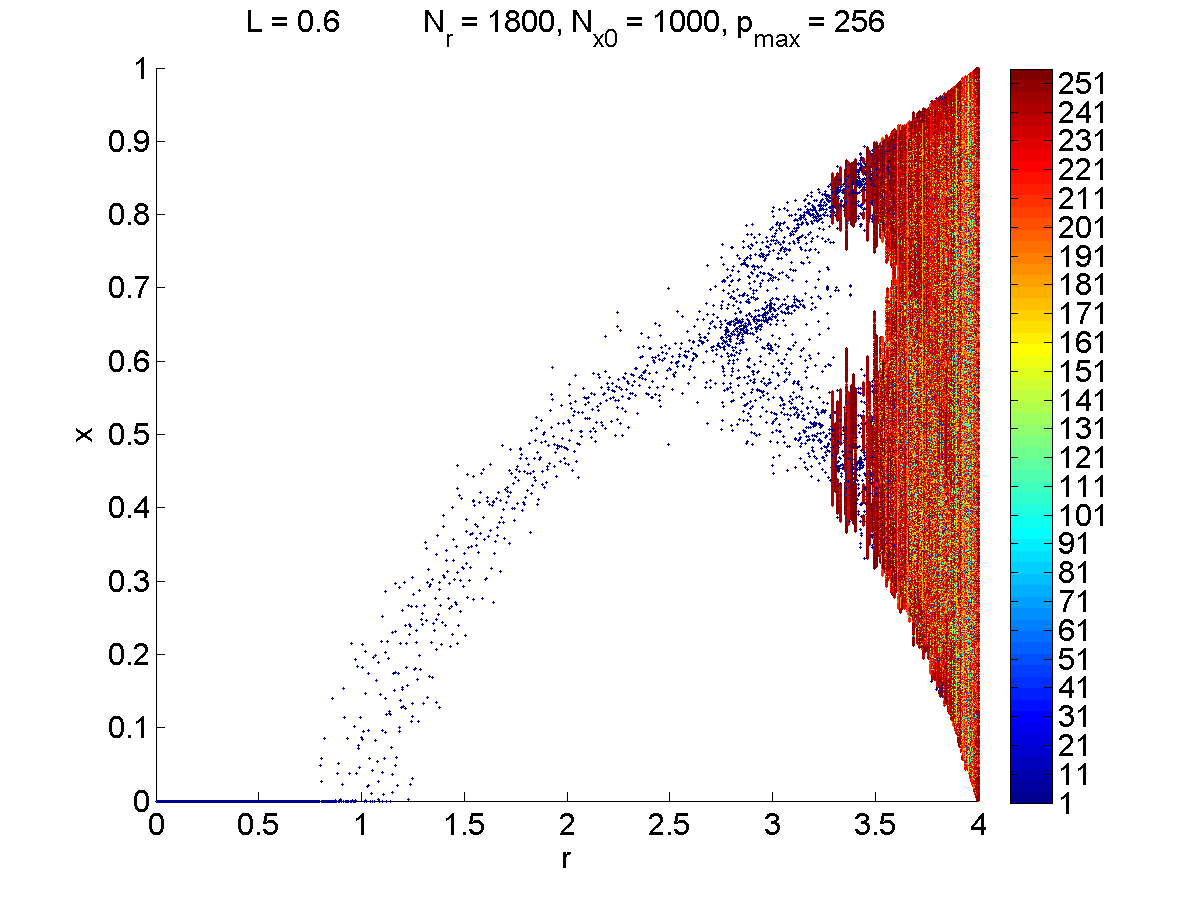
\includegraphics[width=.5\textwidth]{figs/rlog_bif_halfs_L_06.png}\\
		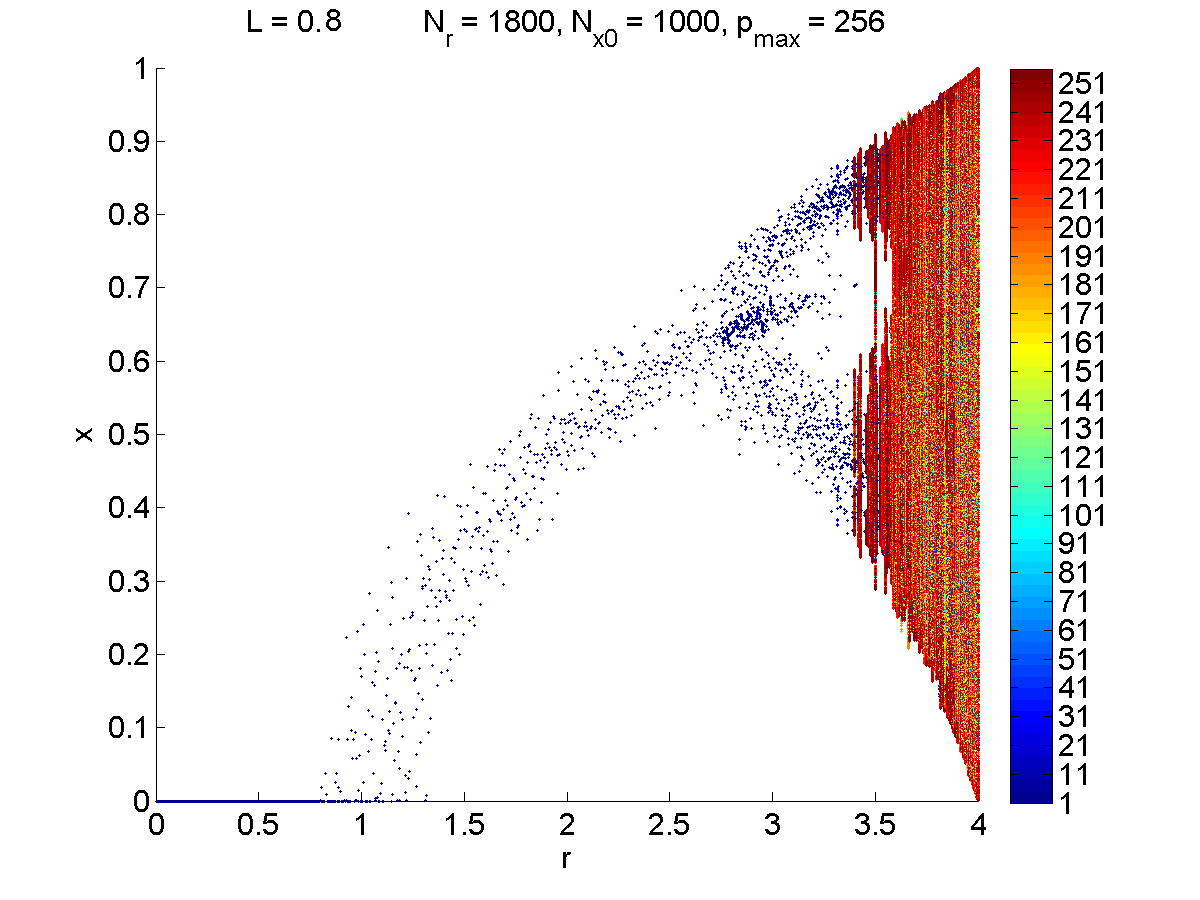
\includegraphics[width=.5\textwidth]{figs/rlog_bif_halfs_L_08.png}\hfill
		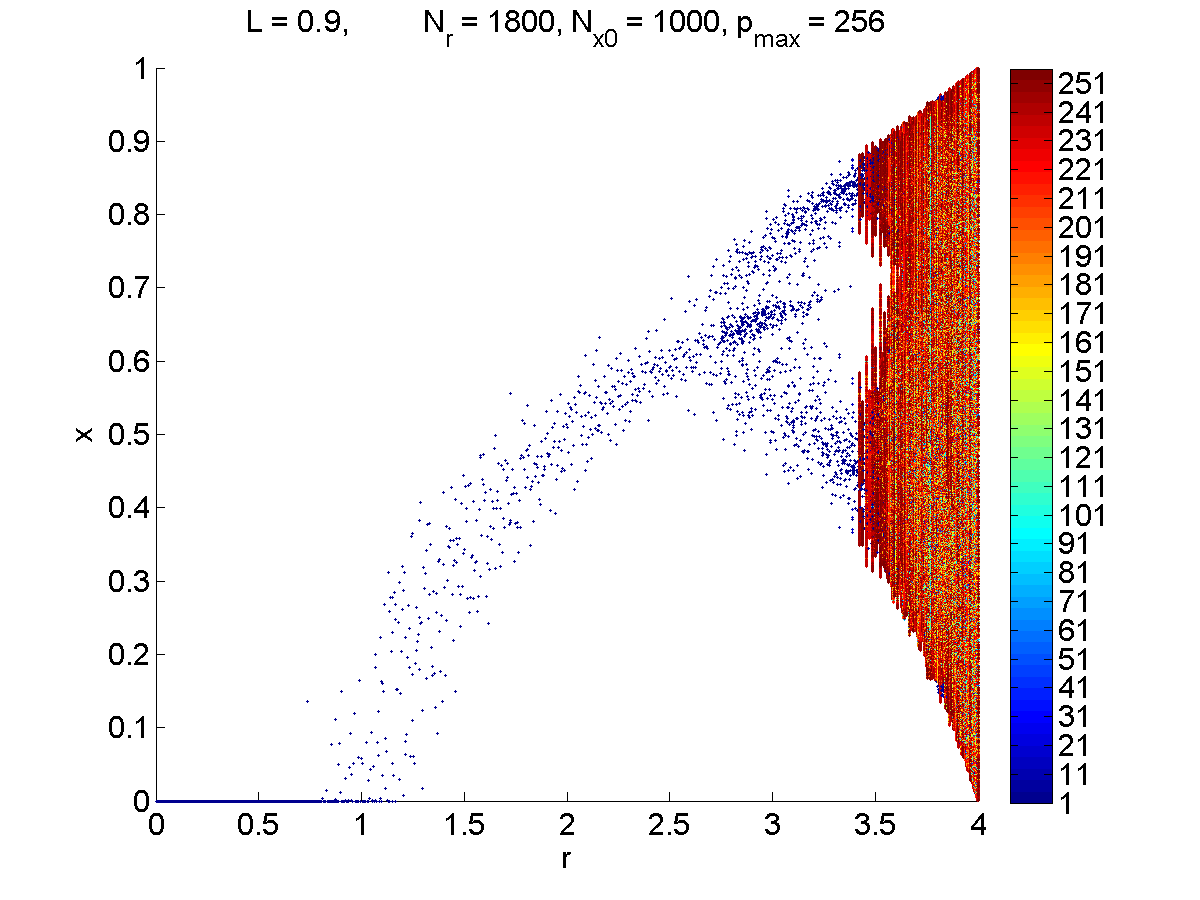
\includegraphics[width=.5\textwidth]{figs/rlog_bif_halfs_L_09.png}\\
	\end{center}
\end{figure}
\begin{figure}[!h]
\caption[Lyapunov exponent in the random logistic map compared to the
deterministic map, $\sigma=\frac{1}{2}\sigma_{max}$]{The Lyapunov exponent for the deterministic
  logistic map (top left) is compared
  to the Lyapunov exponent of the random logistic map for $L \in
  \{0.05,0.1,0.4,0.8,0.9\}$, where $x_0=0.7$ for $r \in [3,4]$, and
  $\sigma$ is chosen to be half of the maximal value in the interval
  from~(\ref{sigma}). The number of exponents computed was $N_\lambda=10,000$. Plots are read left to right, and top to bottom. }\label{fig:rloglyap2_hs}
\centering
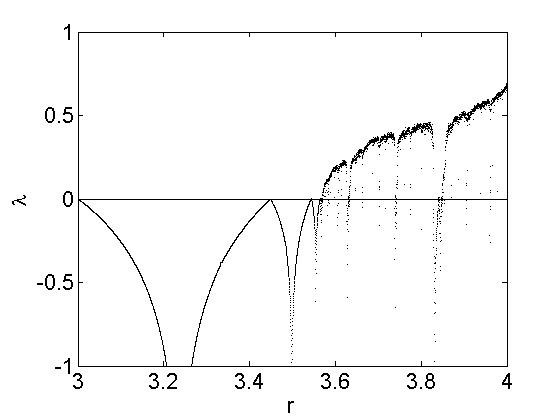
\includegraphics[width=.5\textwidth]{figs/det_log_lyap.png}\hfill
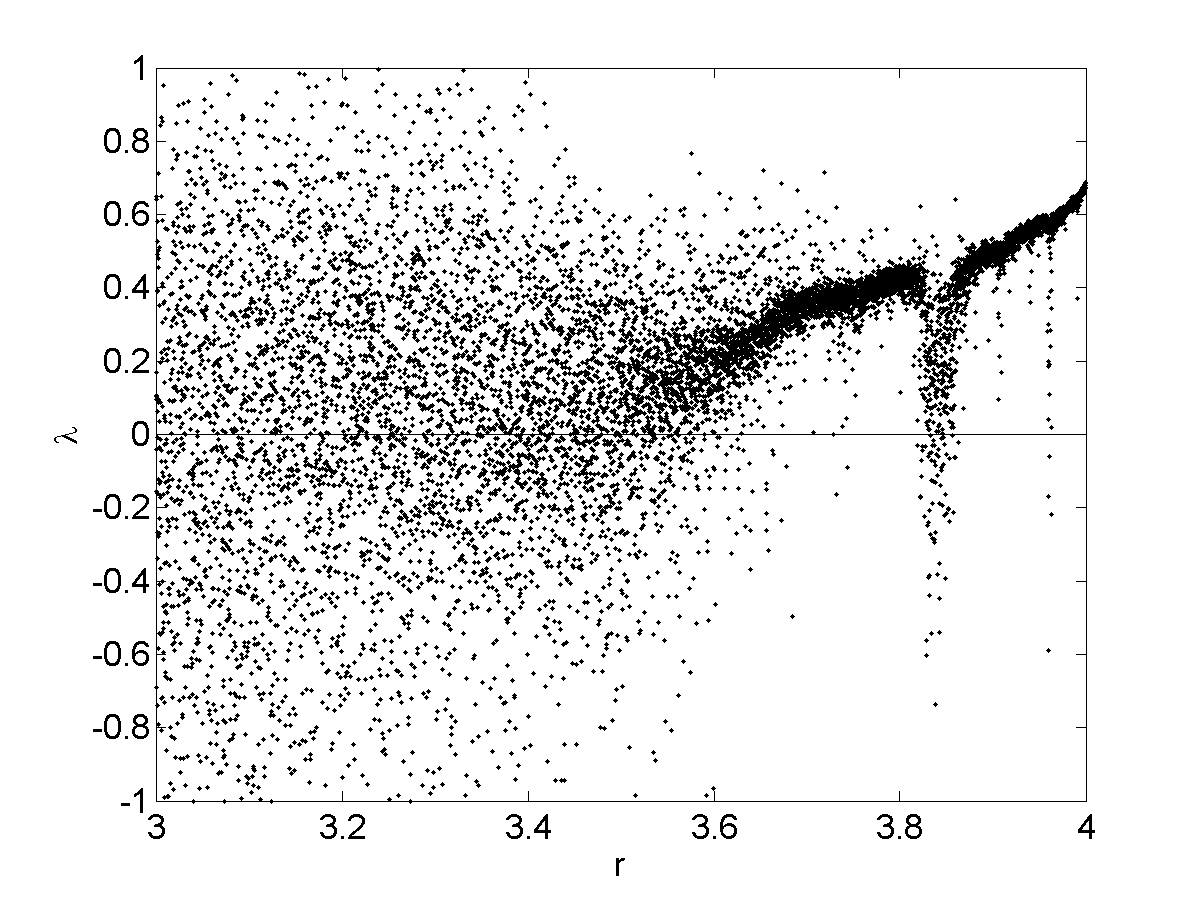
\includegraphics[width=.5\textwidth]{figs/rlog_lyap_halfsig_L_005.png}\\
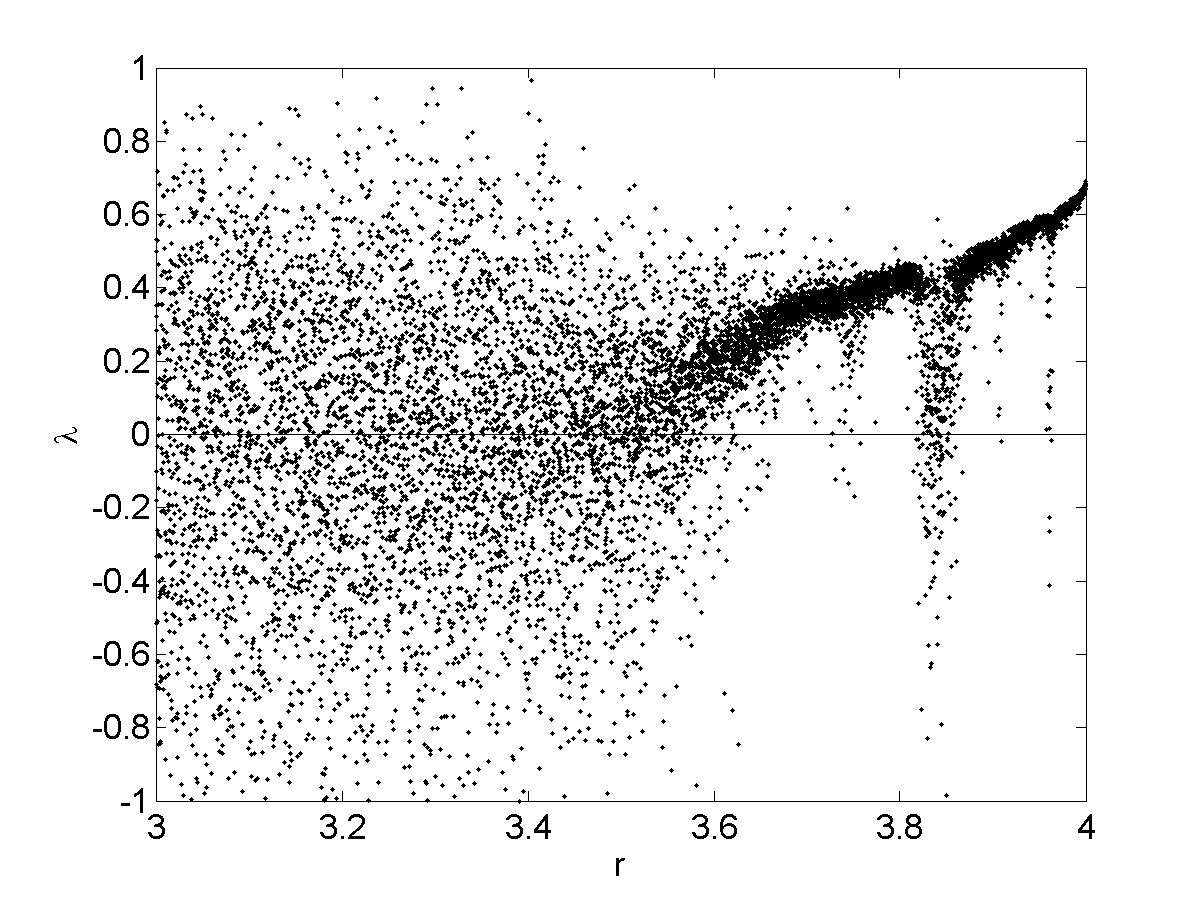
\includegraphics[width=.5\textwidth]{figs/rlog_lyap_halfsig_L_01.png}\hfill
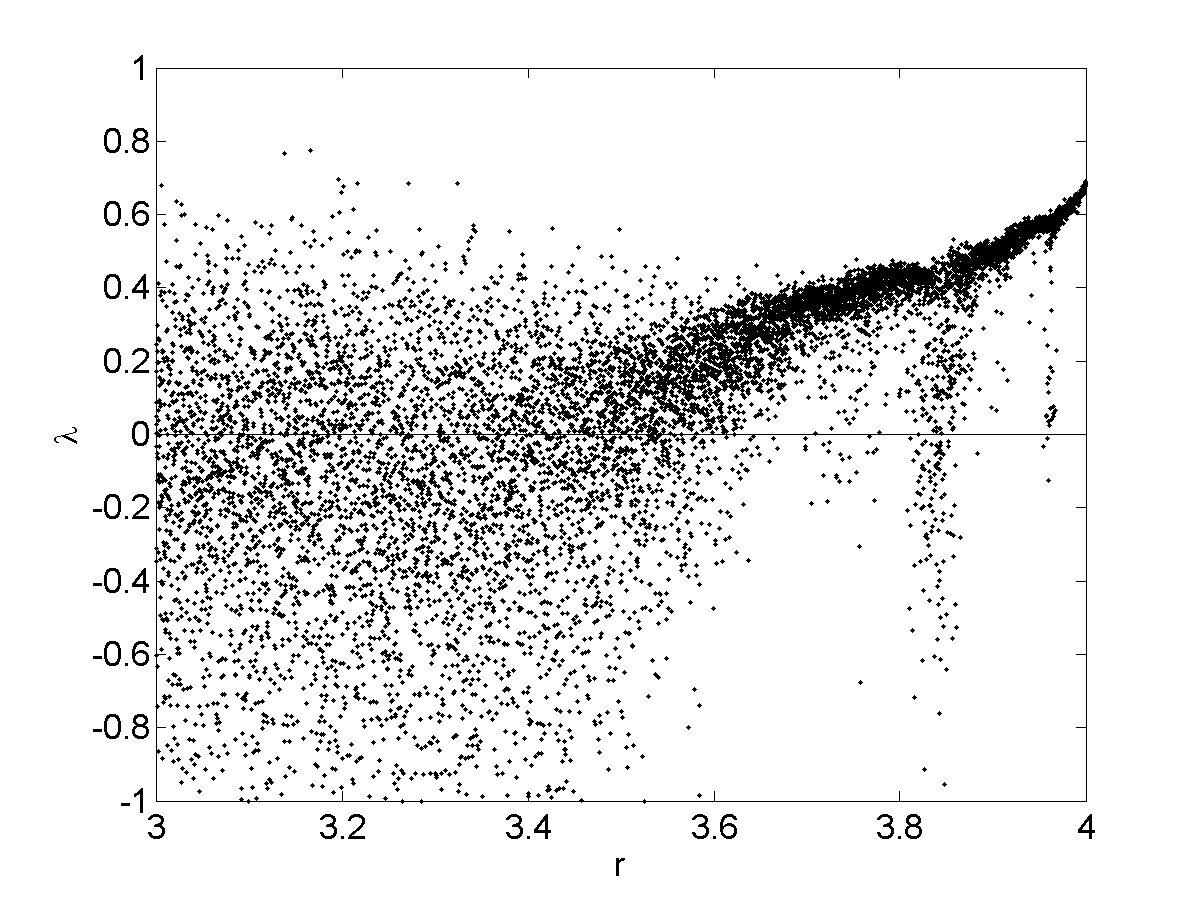
\includegraphics[width=.5\textwidth]{figs/rlog_lyap_halfsig_L_04.png}\\
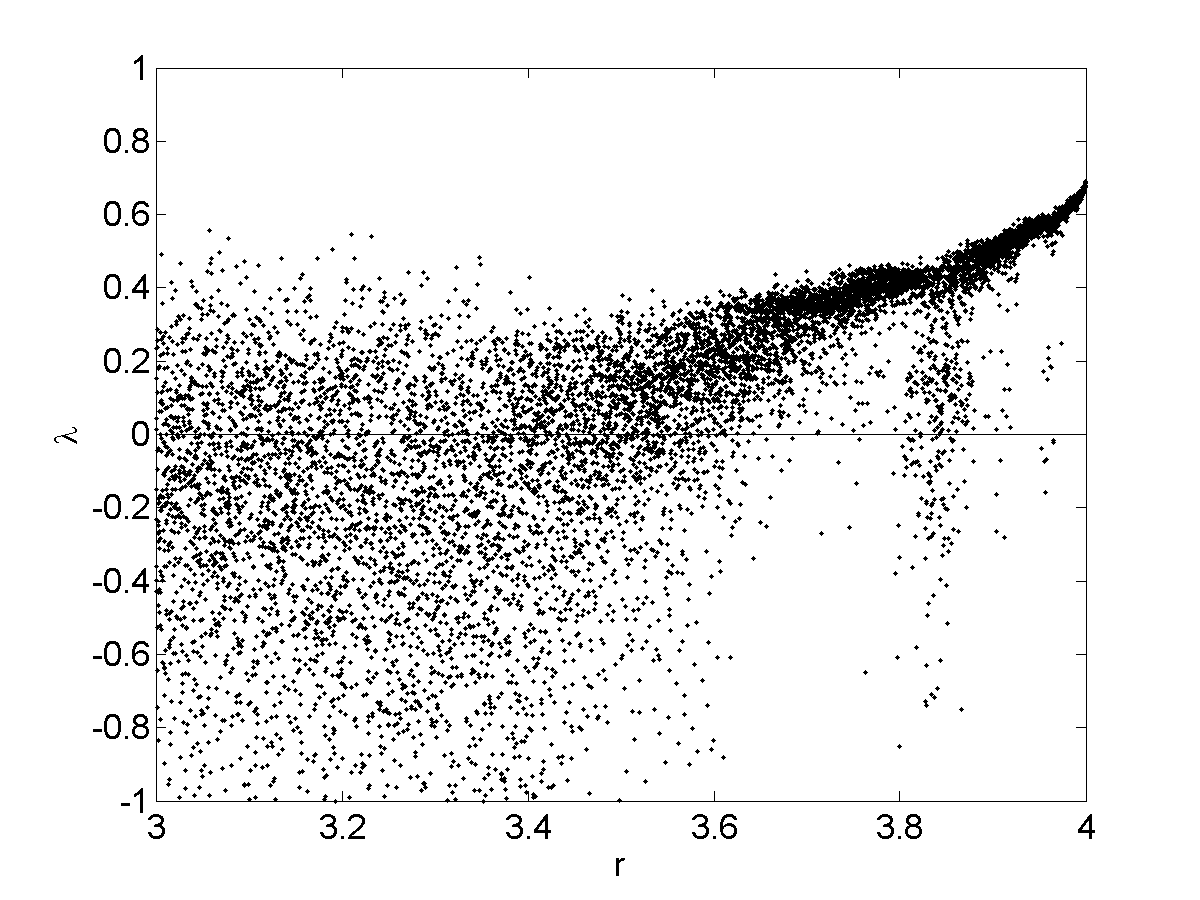
\includegraphics[width=.5\textwidth]{figs/rlog_lyap_halfsig_L_08.png}\hfill
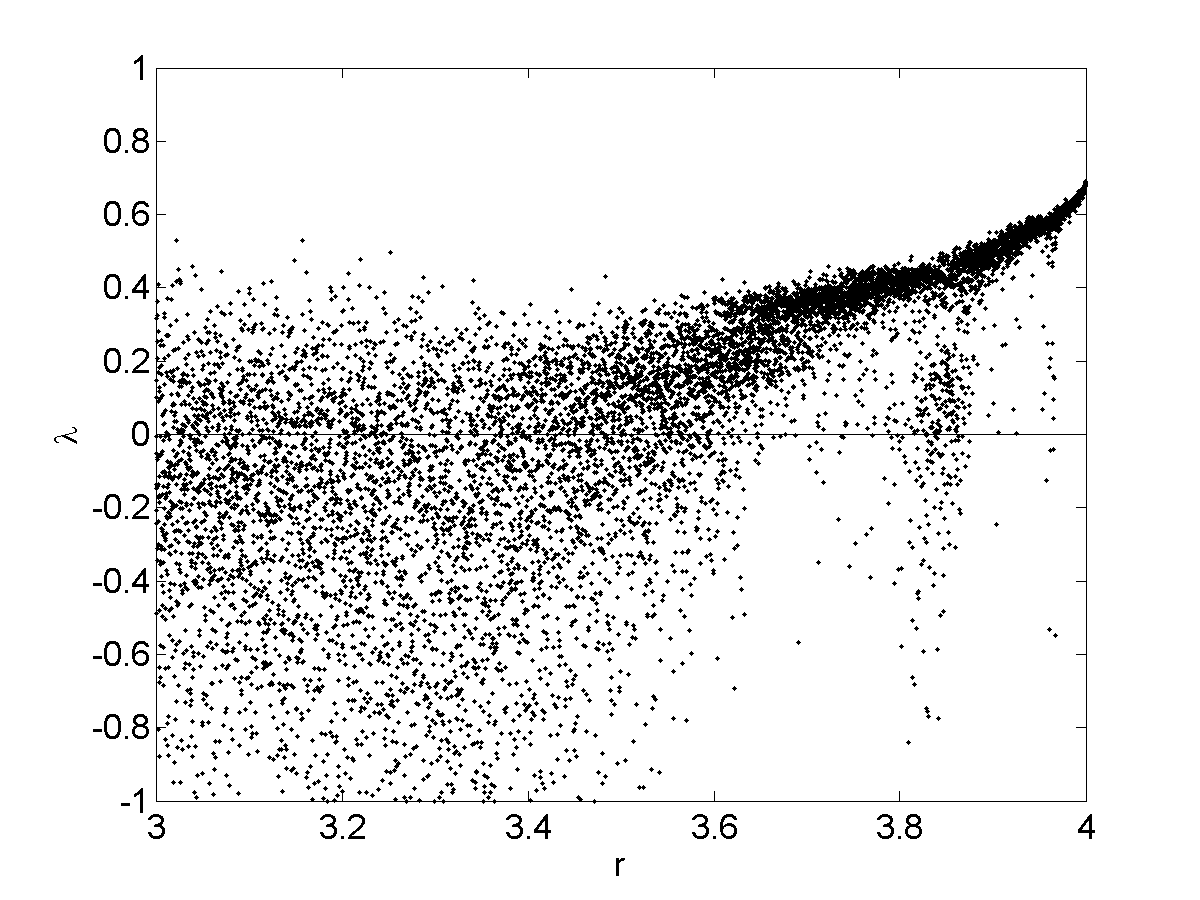
\includegraphics[width=.5\textwidth]{figs/rlog_lyap_halfsig_L_09.png}\\
\end{figure}

\section{Implementation of Randomness in the Circle Map}
We explored how the random circle map for uniformly distributed $\hat{\xi}_n$ and
normally distributed $\hat{\xi}_n$ changes in terms of its Arnold
Tongues, devil's staircases, and Lyapunov exponents. We examined the
distribution of rotation numbers using a kernel density
estimator. The parameter $\alpha$ that scales the variance of the
spatial process $\xi(x)$ was tested for two values: $\alpha=10^{-5}$
and $\alpha = \frac{1}{2}10^{-5}$.
\subsection{Uniform Distribution}
The randomized circle map for uniformly distributed $\hat{\xi}_n$ has a set of Arnold Tongues (Figure~\ref{fig:rcirctongues_u}) that has almost no similarity to the deterministic
case. For low values of $L$, we have lost the
shape of the tongues, and the diagram becomes asymmetrical. For larger
values of $L$, the distinctive tongues and the overall symmetry is
recovered. The randomness appears to have an overall destabilizing
effect on the dynamics of the map. For $L=0.05$, we also observe the
presence of high-period orbits in the region where there is typically
only period 1 fixed points (upper left). As $L$ increases, this region
morphs into predominantly stable period 1 orbits. 

Figure~\ref{fig:rcirclyap_u} is a plot of the Lyapunov
exponents for a fixed $k$ and varying $\omega$, whereas
Figure~\ref{fig:rcirclyap2_u} fixes $\omega$ and varies $k$. A comparison of the Lyapunov exponent of the deterministic and random
case (Figure~\ref{fig:rcirclyap_u} and Figure~\ref{fig:rcirclyap2_u})
partially confirms the idea that the noise is destabilizing; nearly no
features of the deterministic graph are preserved (for small $L$), and the high
density of positive values indicates chaotic
behavior. Moreover,
Figure~\ref{fig:rcirclyap_u} demonstrates that there is a skewed
distribution of Lyapunov exponents on the right side of the graph for
all values of $L$, compared to the left side. However, this trend is not observed in Figure~\ref{fig:rcirclyap2_u}.

% In Figure~\ref{fig:rcirc_bifw_u}, it appears that as $\omega$ is
% varied over $[0,1]$ (for fixed $k=1$), the distribution of stable
% orbits follows the line $x=\omega$. However, closer examination of the
% solutions of (\ref{randcirc}) demonstrate
% \begin{align*}
% \begin{split}
% \omega &= \frac{k}{2\pi}\sin(2\pi x)\\
% x &= \frac{1}{2\pi}\arcsin\left(\frac{2\pi \omega}{k}\right).
% \end{split}
% \end{align*}

\begin{figure}[H]\linespread{1}  
\caption[The Arnold tongues for the random circle map, uniform
distribution, $\alpha = 10^{-5}$]{The Arnold
  tongues for $k\in [0,1.5]$, $\Delta k = 0.0015$, $\omega \in [0,1]$,
  $\Delta \omega = 0.001$, $\alpha = 10^{-5}$, $\hat{\xi}_n\sim Unif(-M_n,M_n)$ and $L_j \in
  \{0.05,0.1,0.3,0.5,0.7,0.9\}$. $\Delta k$ and $\Delta \omega$
  represent the step size in discretizing $k$ on [0,1.5] and $\omega$
  on [0,1]. Plots are ordered left to right,
  and top to bottom. The colorbar to the right demonstrates the period and corresponding color.}\label{fig:rcirctongues_u}
\centering
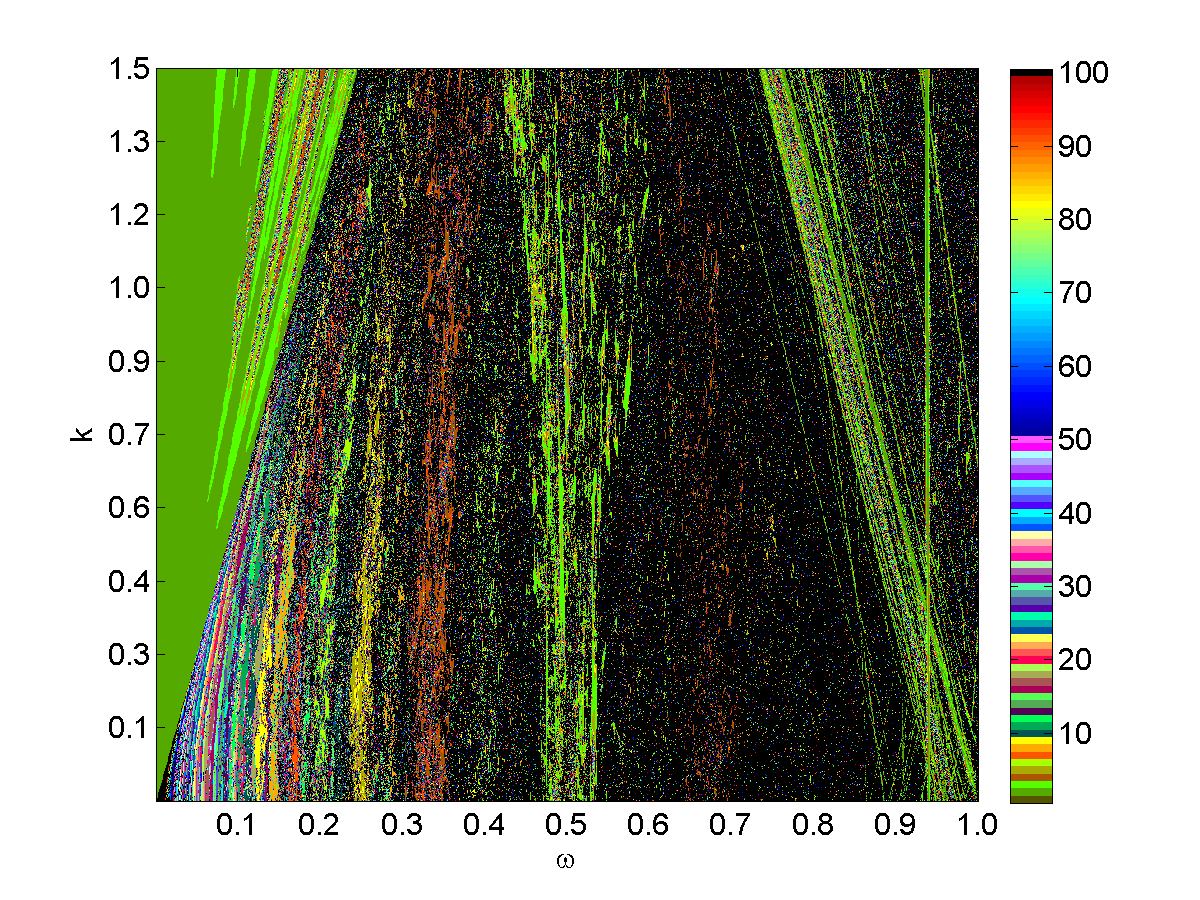
\includegraphics[width=.5\textwidth]{figs/tongues_1000_L_005.png}\hfill
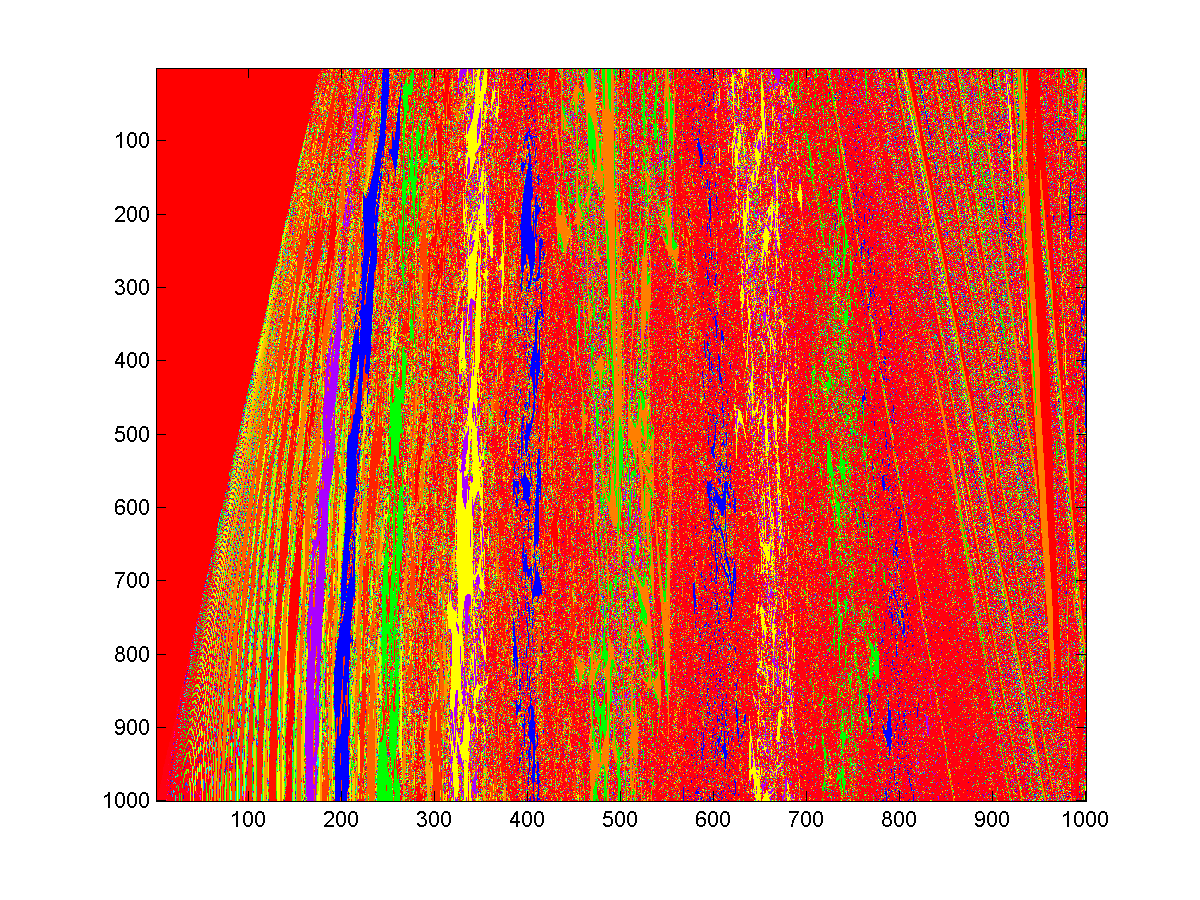
\includegraphics[width=.5\textwidth]{figs/tongues_1000_L_01.png}\\
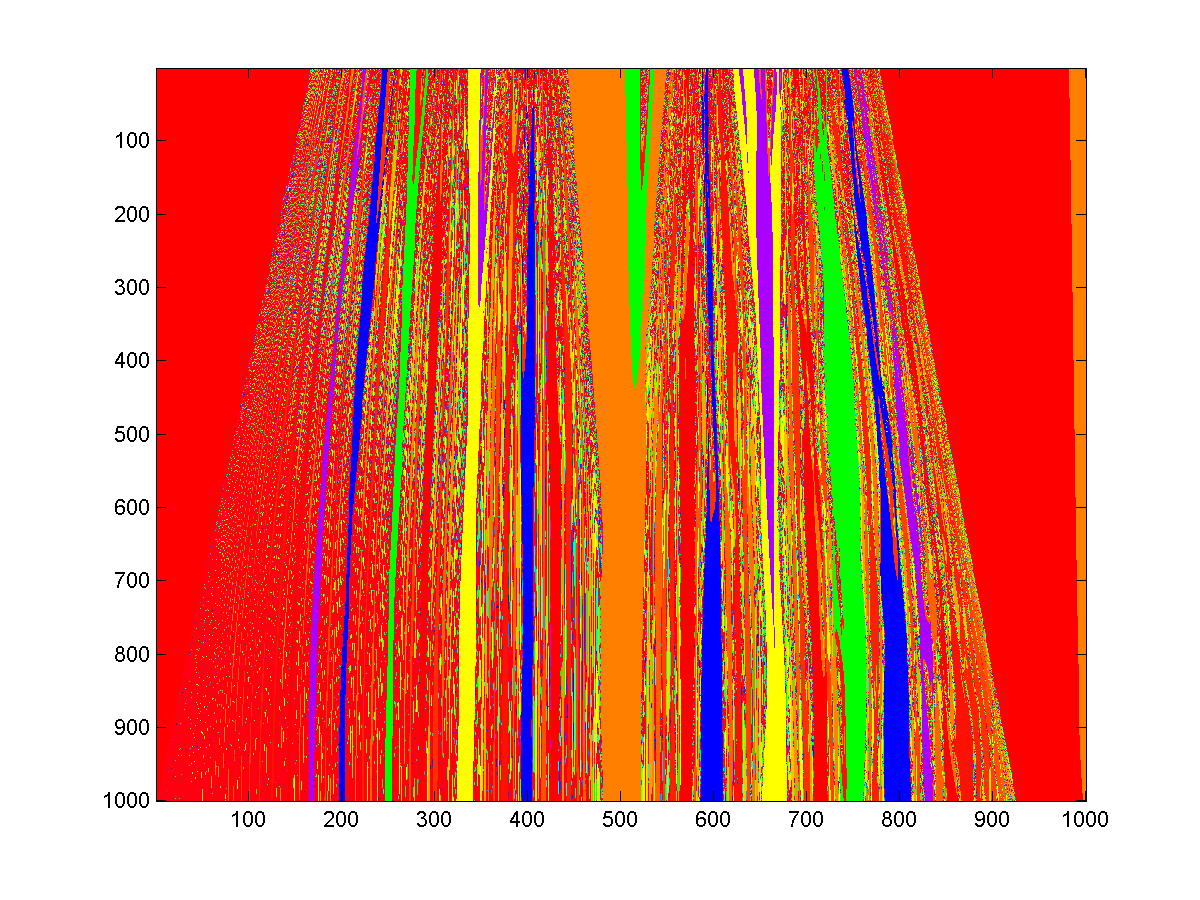
\includegraphics[width=.5\textwidth]{figs/tongues_1000_L_03.png}\hfill
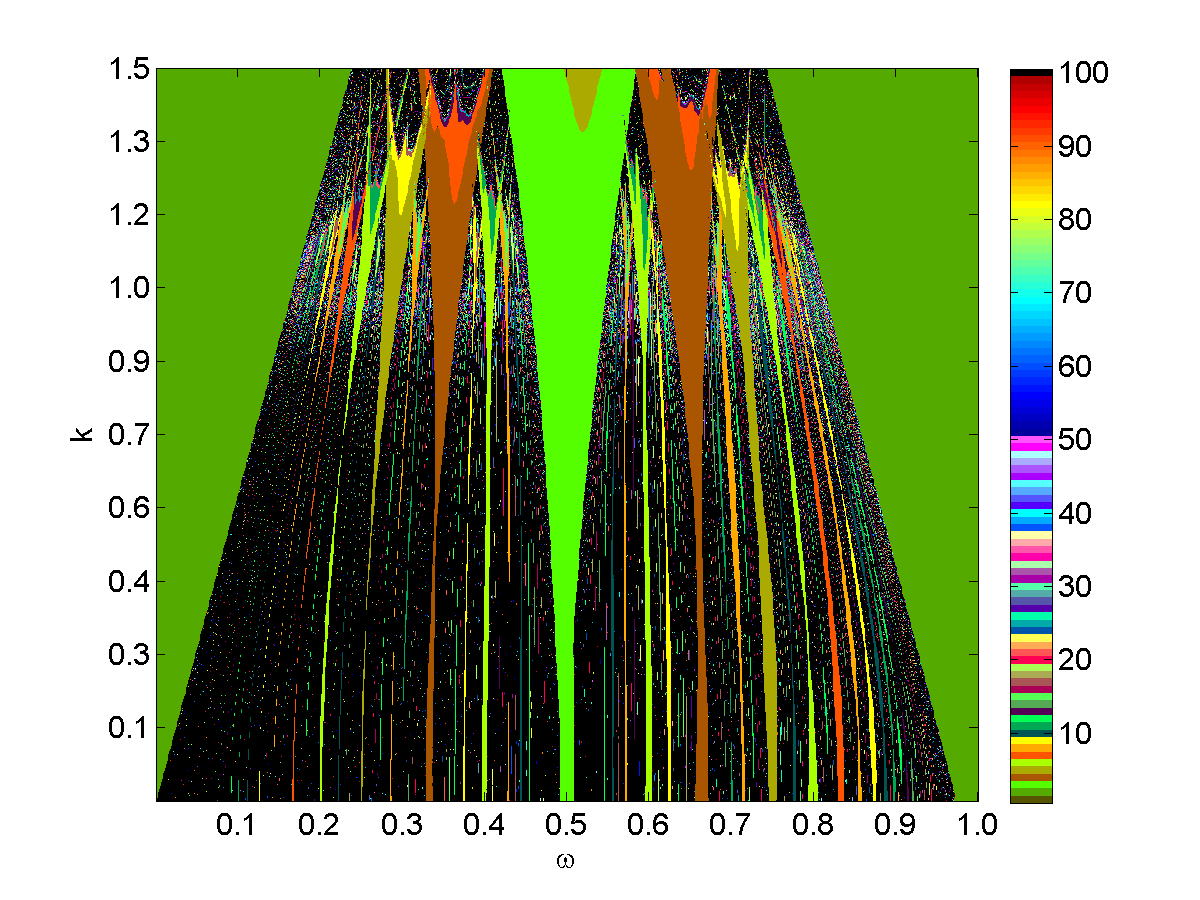
\includegraphics[width=.5\textwidth]{figs/tongues_1000_L_05.png}\\
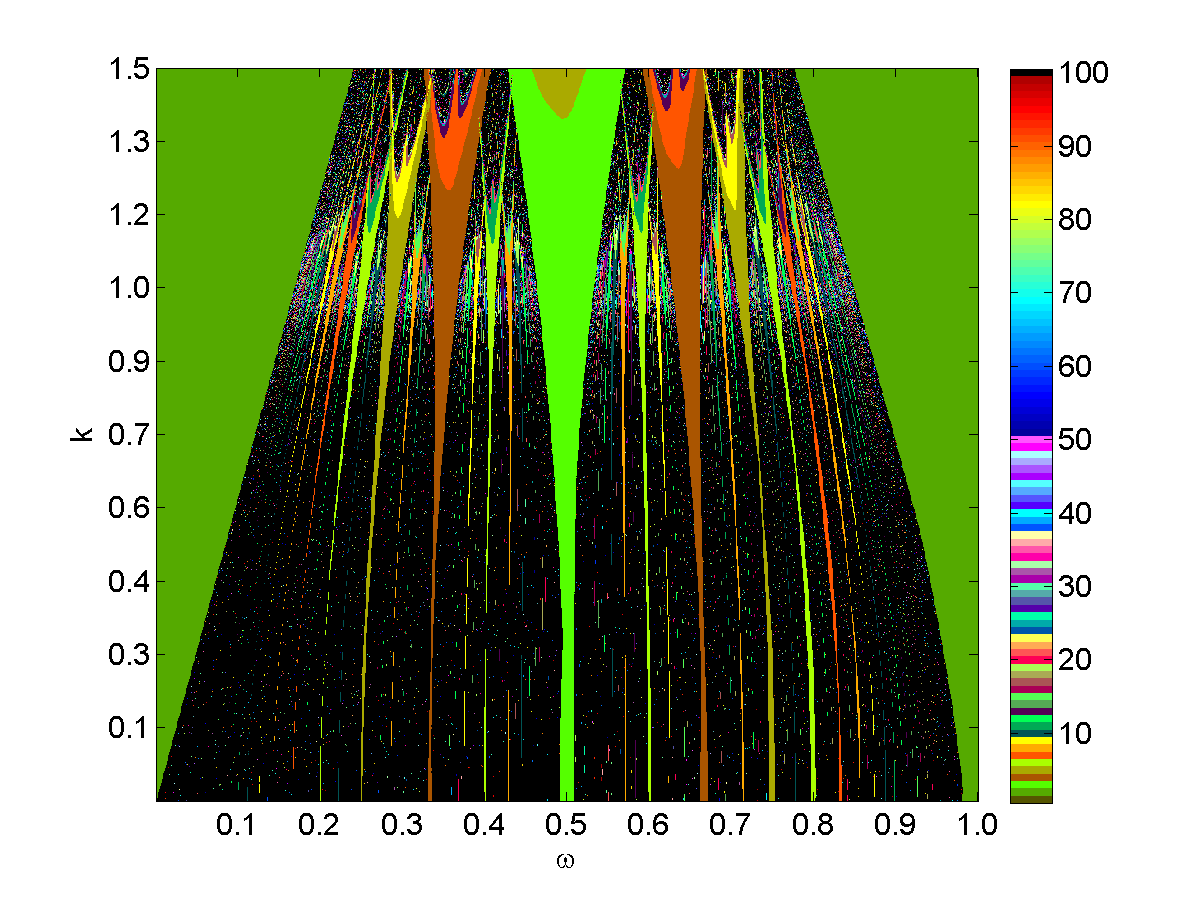
\includegraphics[width=.5\textwidth]{figs/tongues_1000_L_07.png}\hfill
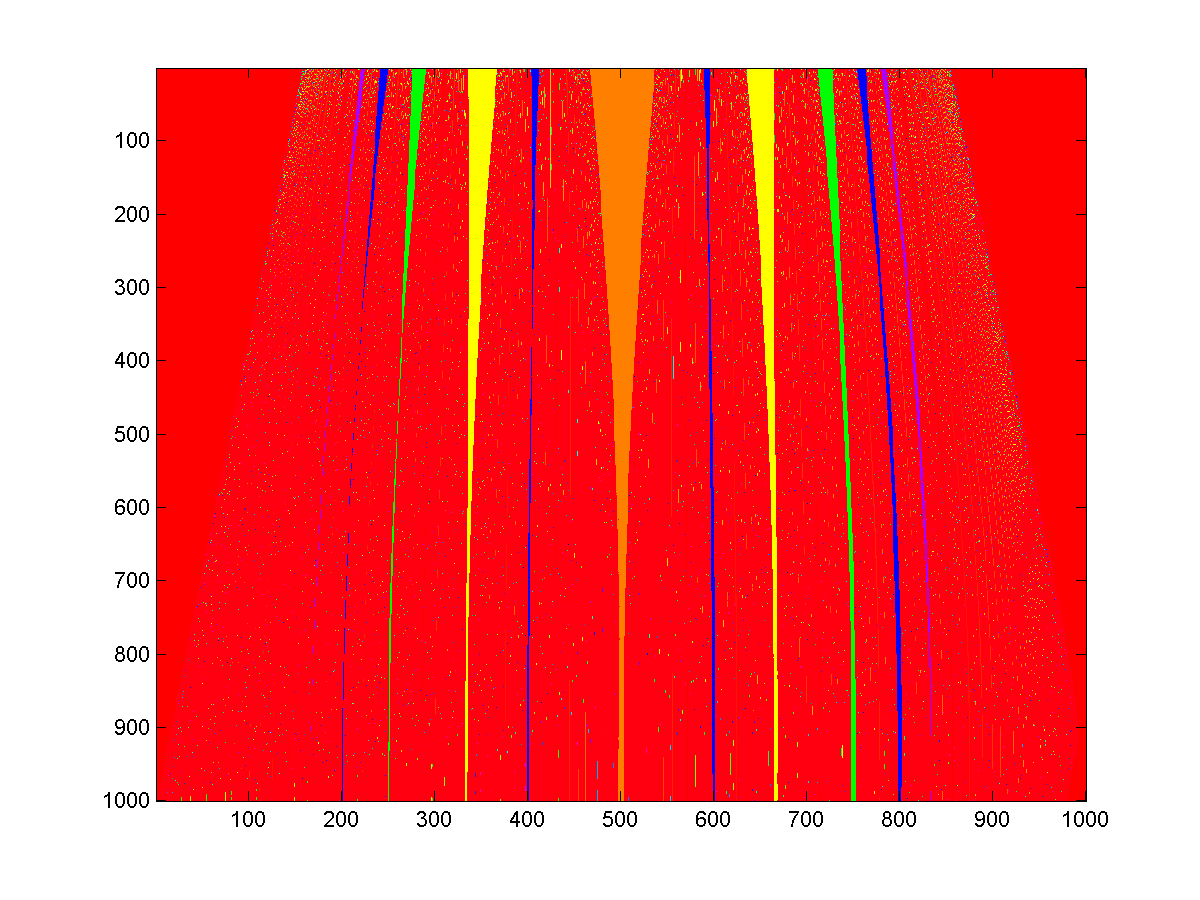
\includegraphics[width=.5\textwidth]{figs/tongues_1000_L_09.png}\\
\end{figure}

\begin{figure}[!h]
\caption[Lyapunov exponent in the random circle map (uniform distribution) compared to the
deterministic map, varying $\omega$, $\alpha = 10^{-5}$]{The Lyapunov exponent for the deterministic
  circle map (top left) is compared
  to the Lyapunov exponent of the random circle map for $L \in
  \{0.05,0.1,0.3,0.5,0.9\}$, where $x_0=0.7$, $k=2$,$\alpha =
  10^{-5}$, and $\hat{\xi}_n\sim
  Unif(-M_n,M_n)$ for $\omega \in [0,1]$. The number of exponents computed was $N_\lambda=10,000$. Plots are read left to right, and top to bottom. }\label{fig:rcirclyap_u}
\centering
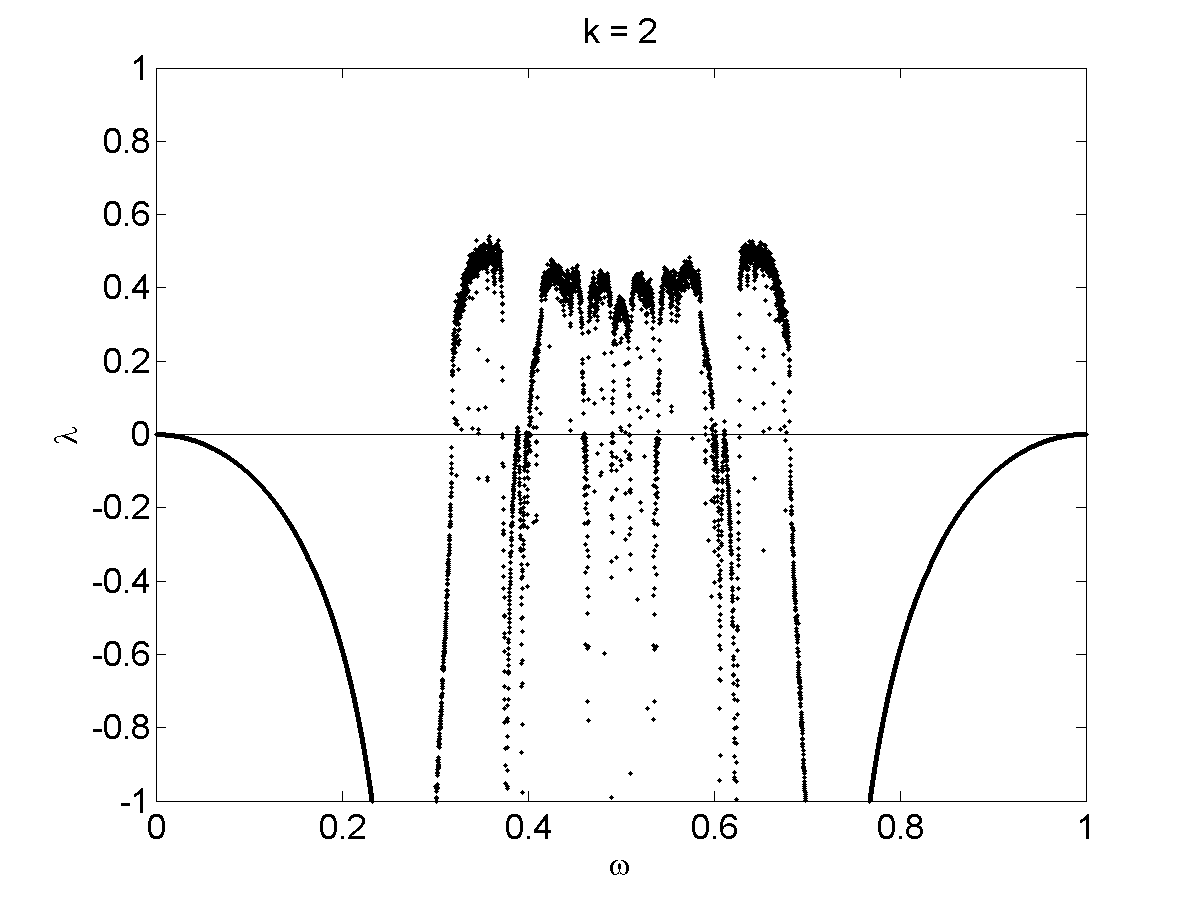
\includegraphics[width=.5\textwidth]{figs/detcirc_lyap_10000_k_2_w.png}\hfill
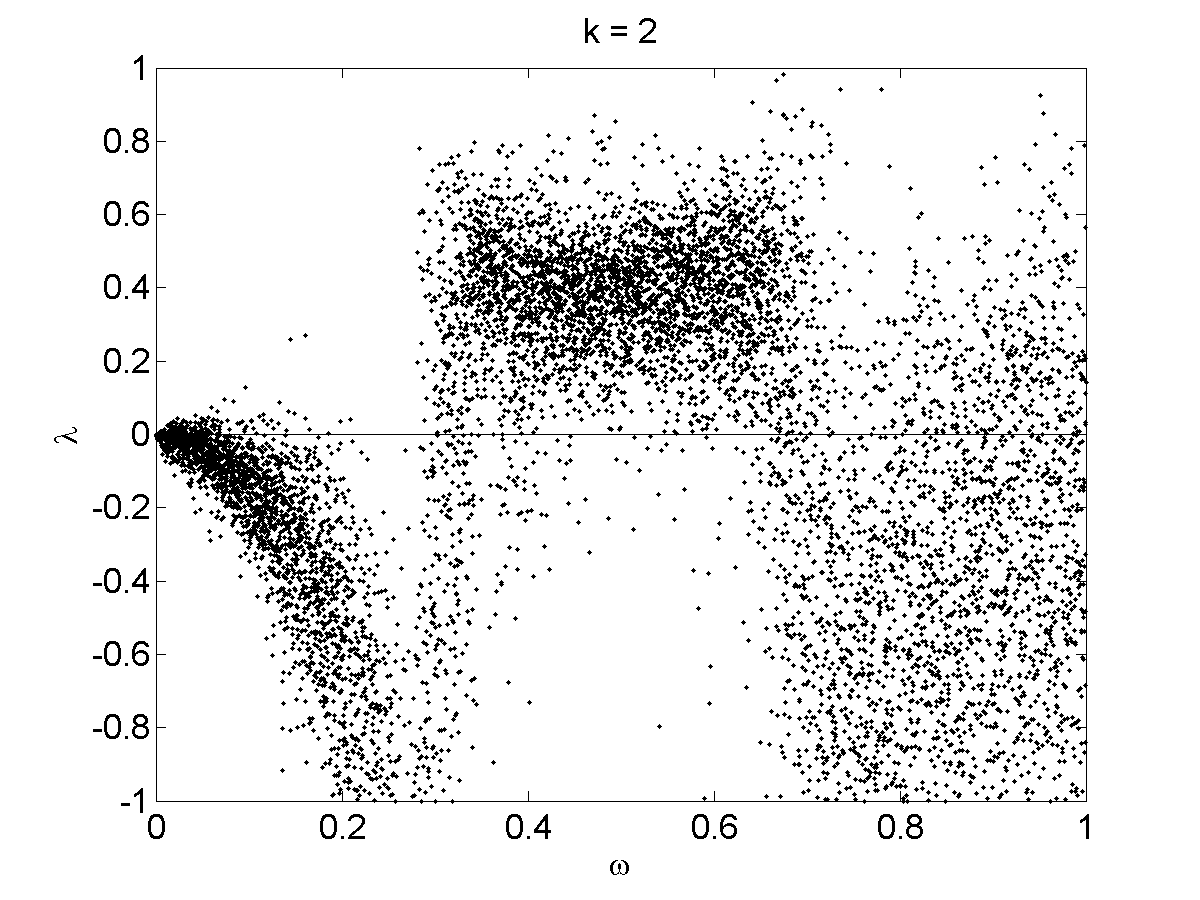
\includegraphics[width=.5\textwidth]{figs/rcirc_u_lyap_10000_L_005_k_2_w.png}\\
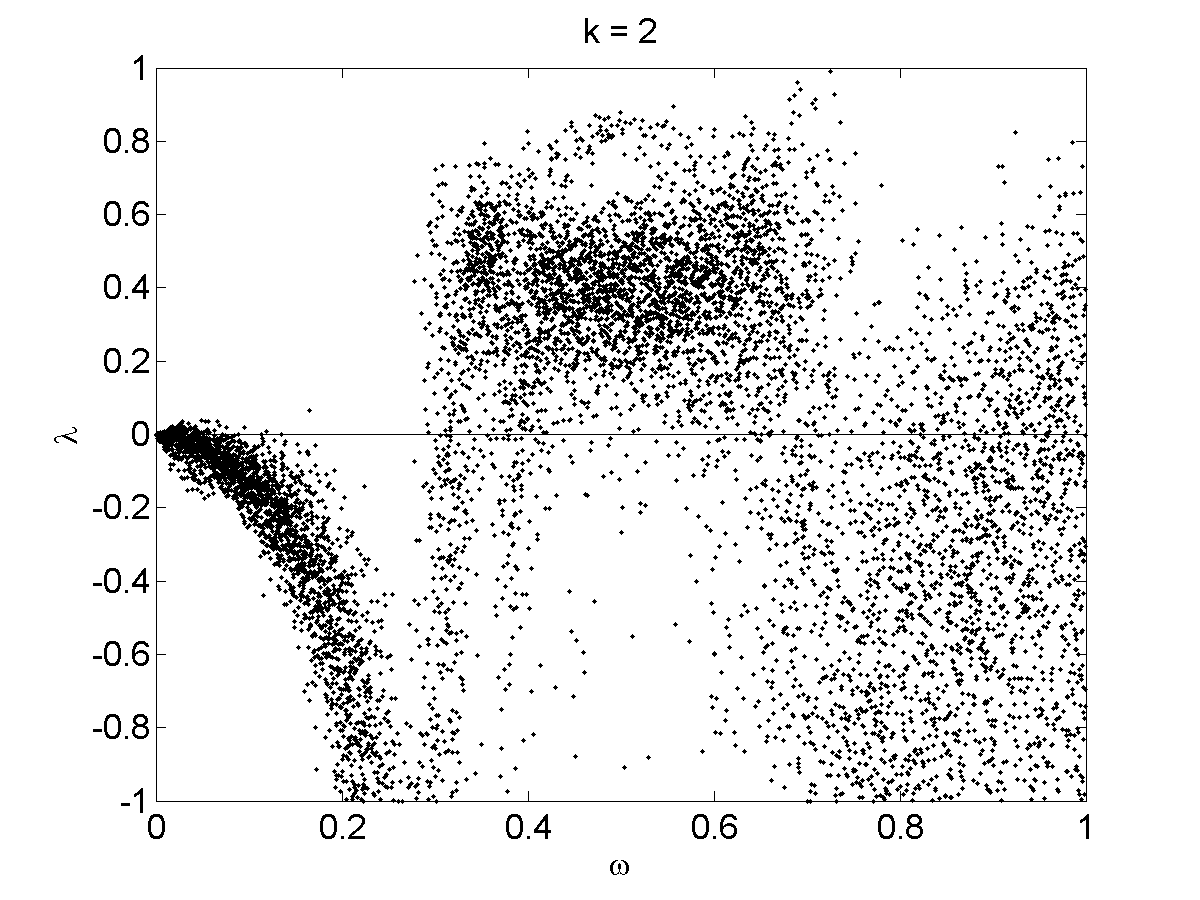
\includegraphics[width=.5\textwidth]{figs/rcirc_u_lyap_10000_L_01_k_2_w.png}\hfill
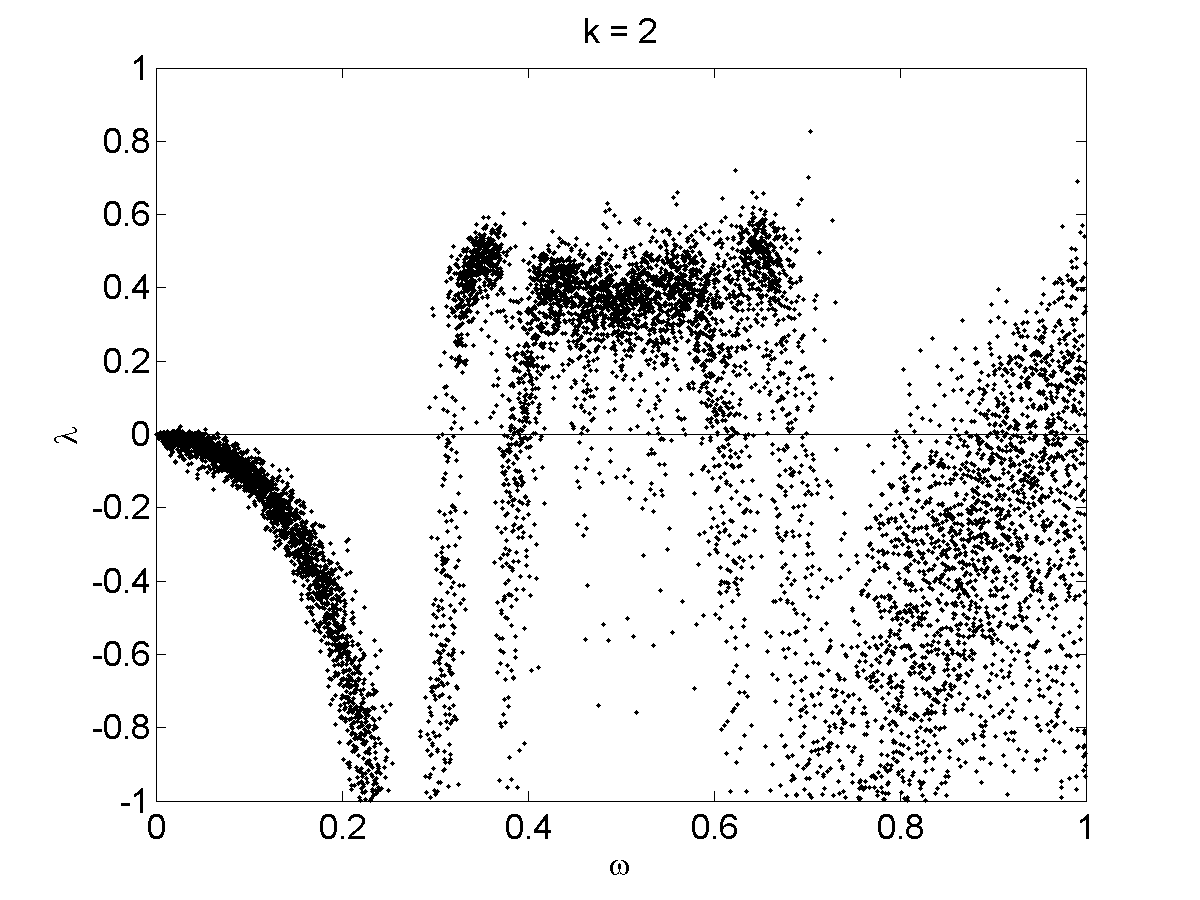
\includegraphics[width=.5\textwidth]{figs/rcirc_u_lyap_10000_L_03_k_2_w.png}\\
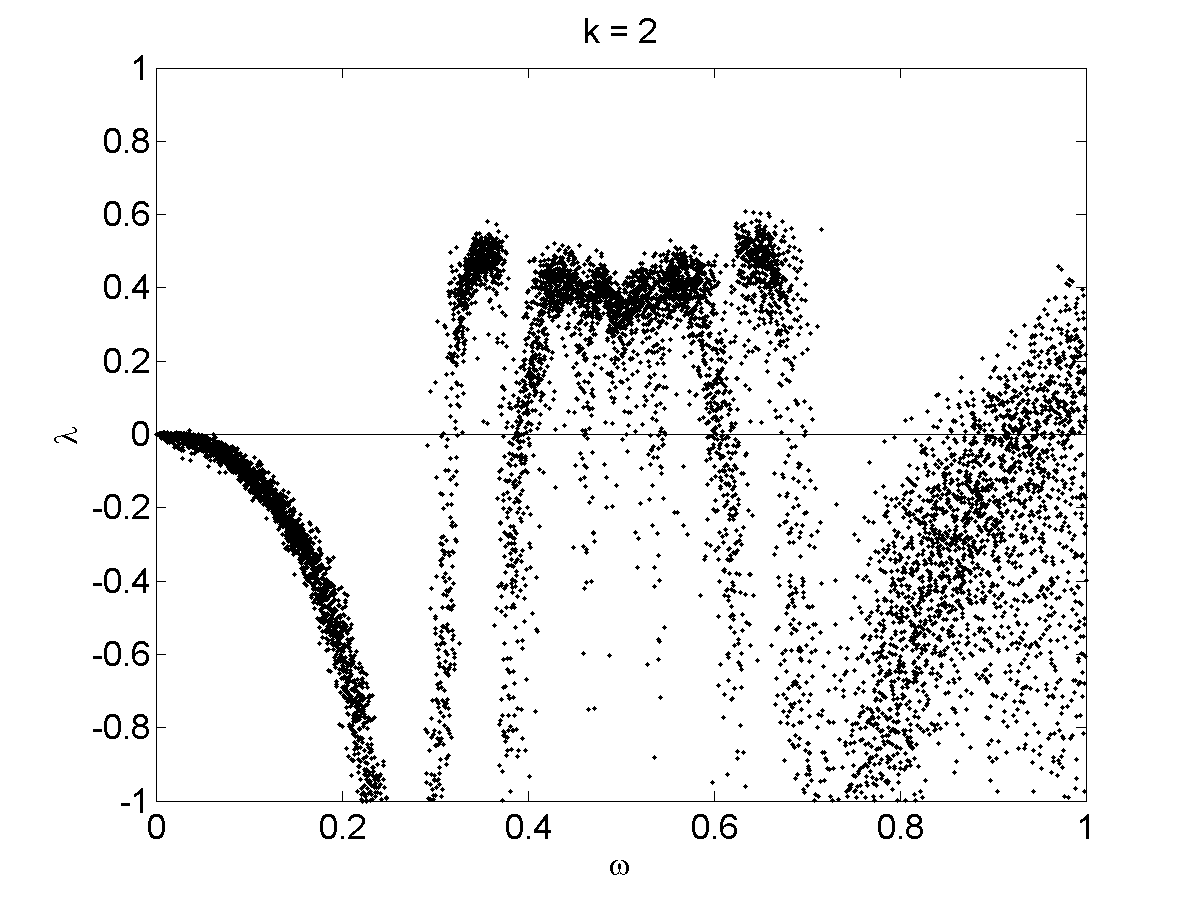
\includegraphics[width=.5\textwidth]{figs/rcirc_u_lyap_10000_L_05_k_2_w.png}\hfill
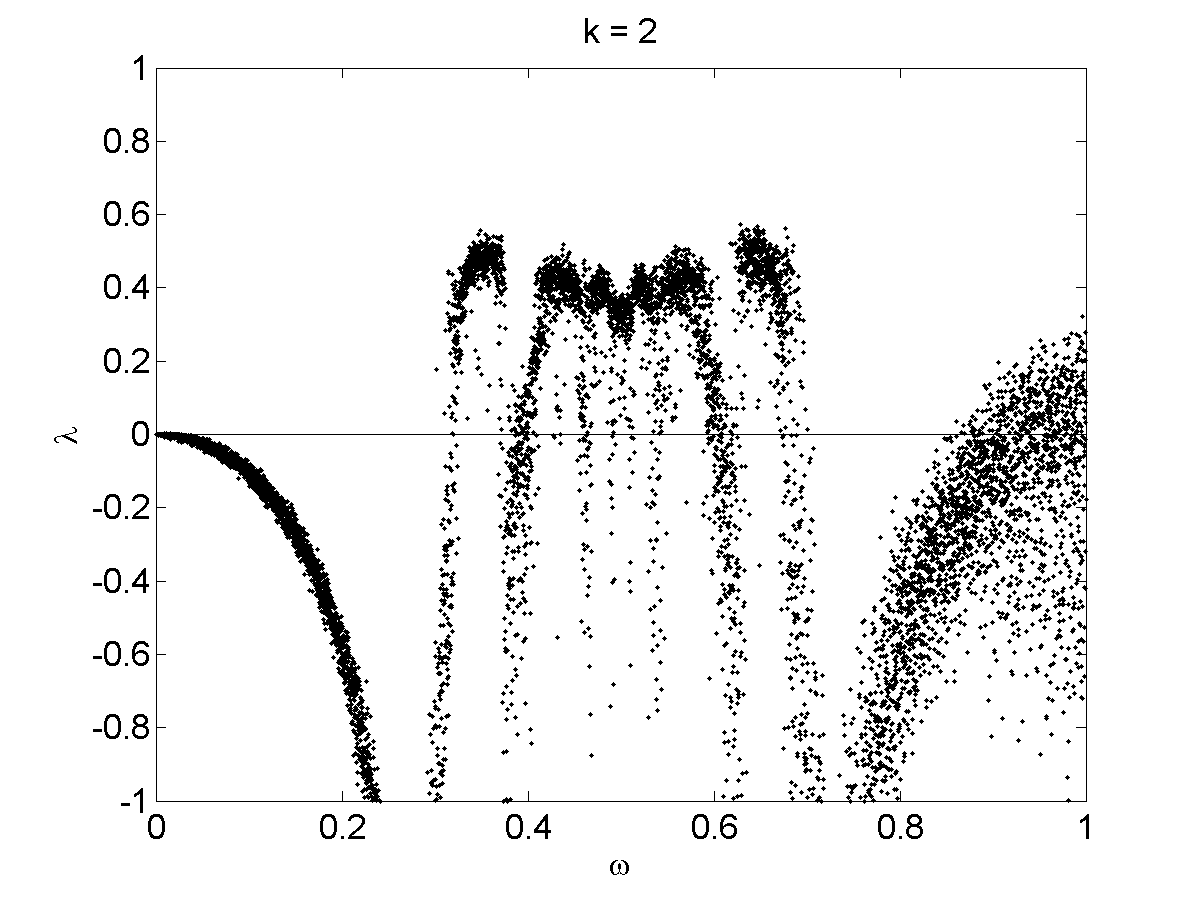
\includegraphics[width=.5\textwidth]{figs/rcirc_u_lyap_10000_L_09_k_2_w.png}\\
\end{figure}

\begin{figure}[!h]
\caption[Lyapunov exponent in the random circle map (uniform distribution) compared to the
deterministic map, varying $k$, $\alpha = 10^{-5}$]{The Lyapunov exponent for the deterministic
  circle map (top left) is compared to the Lyapunov exponent of the random circle map for $L \in \{0.05,0.1,0.3,0.5,0.7\}$, where $x_0=0.7$, $\omega=0.8$,$\alpha = 10^{-5}$, and $\hat{\xi}_n\sim Unif(-M_n,M_n)$ for $k \in [0,5]$. The number of exponents computed was $N_\lambda=10,000$. Plots are read left to right, and top to bottom. }\label{fig:rcirclyap2_u}
\centering
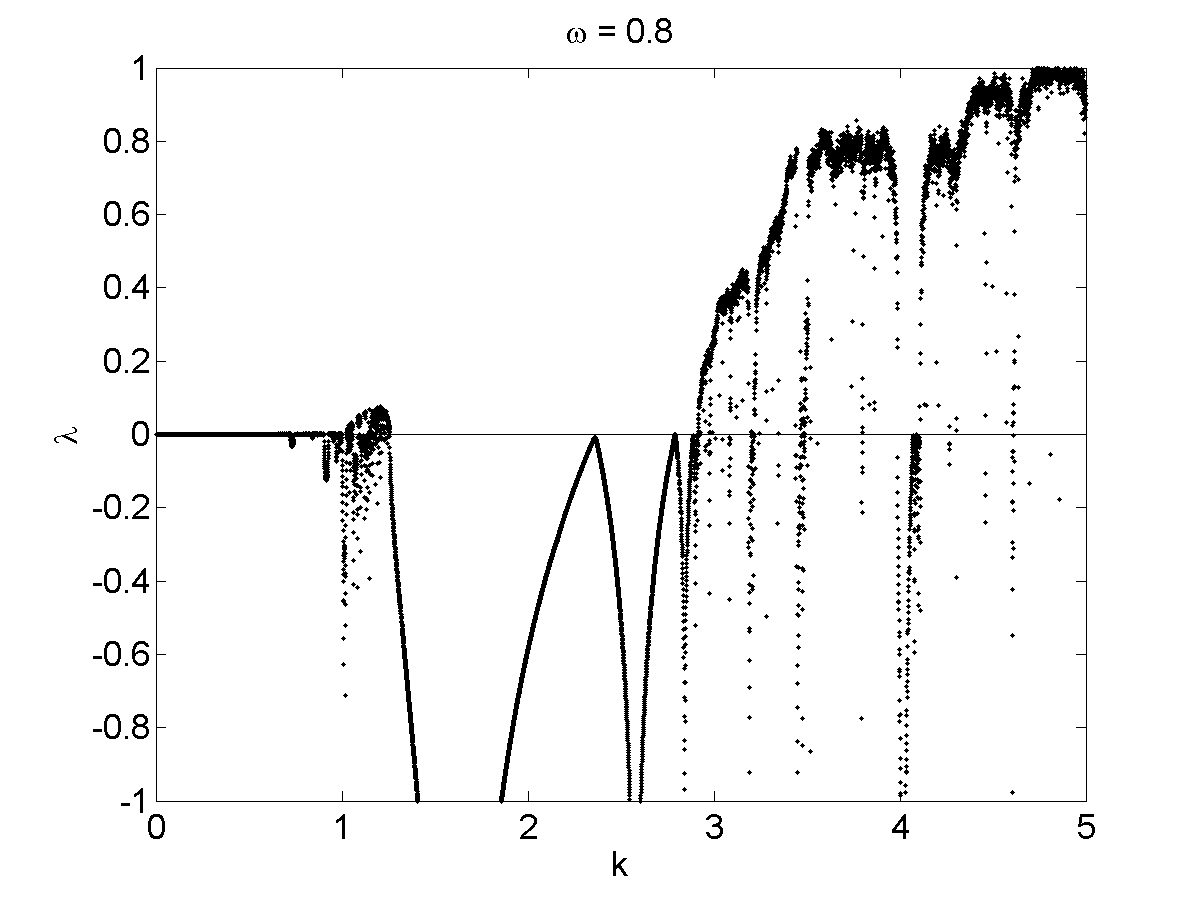
\includegraphics[width=.5\textwidth]{figs/detcirc_n_lyap_10000_w_08_k.png}\hfill
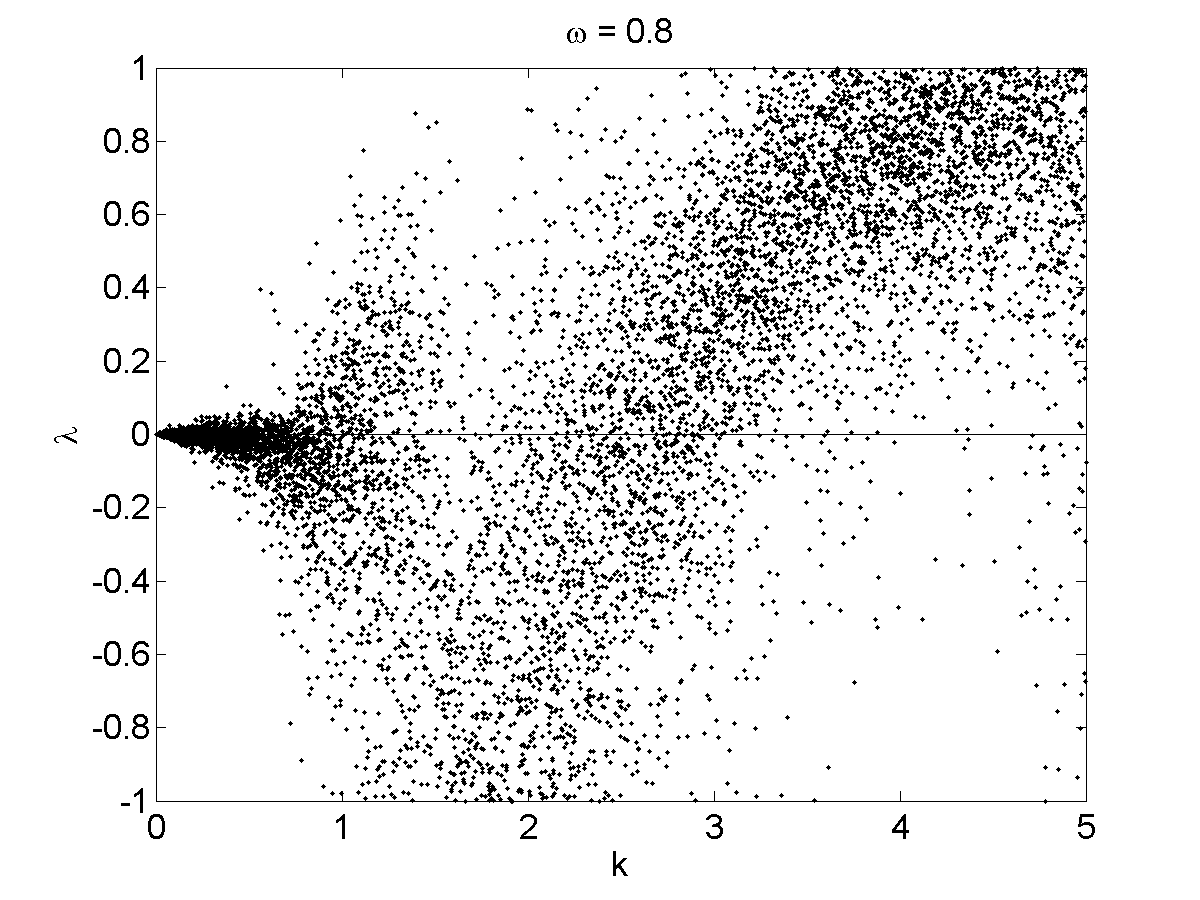
\includegraphics[width=.5\textwidth]{figs/rcirc_u_lyap_10000_L_005_w_08_k.png}\\
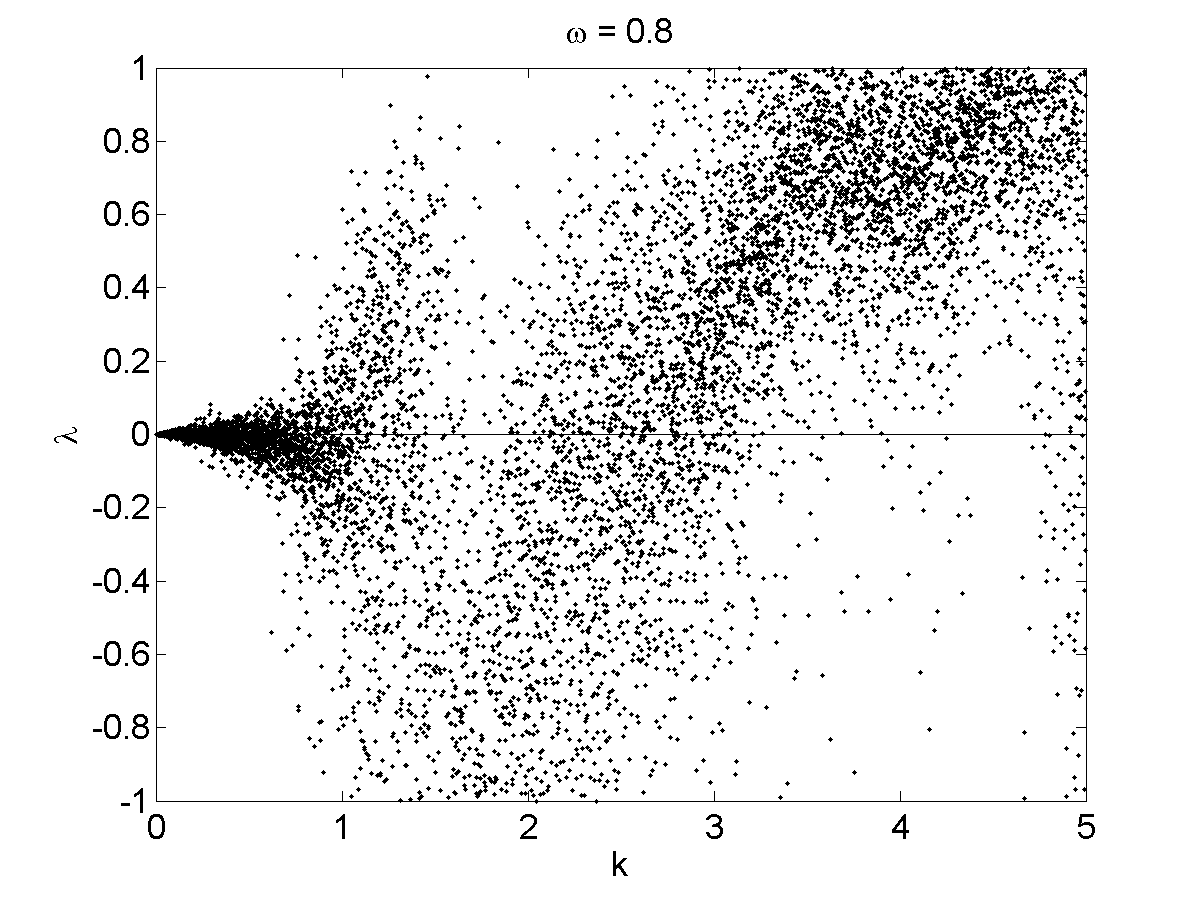
\includegraphics[width=.5\textwidth]{figs/rcirc_u_lyap_10000_L_01_w_08_k.png}\hfill
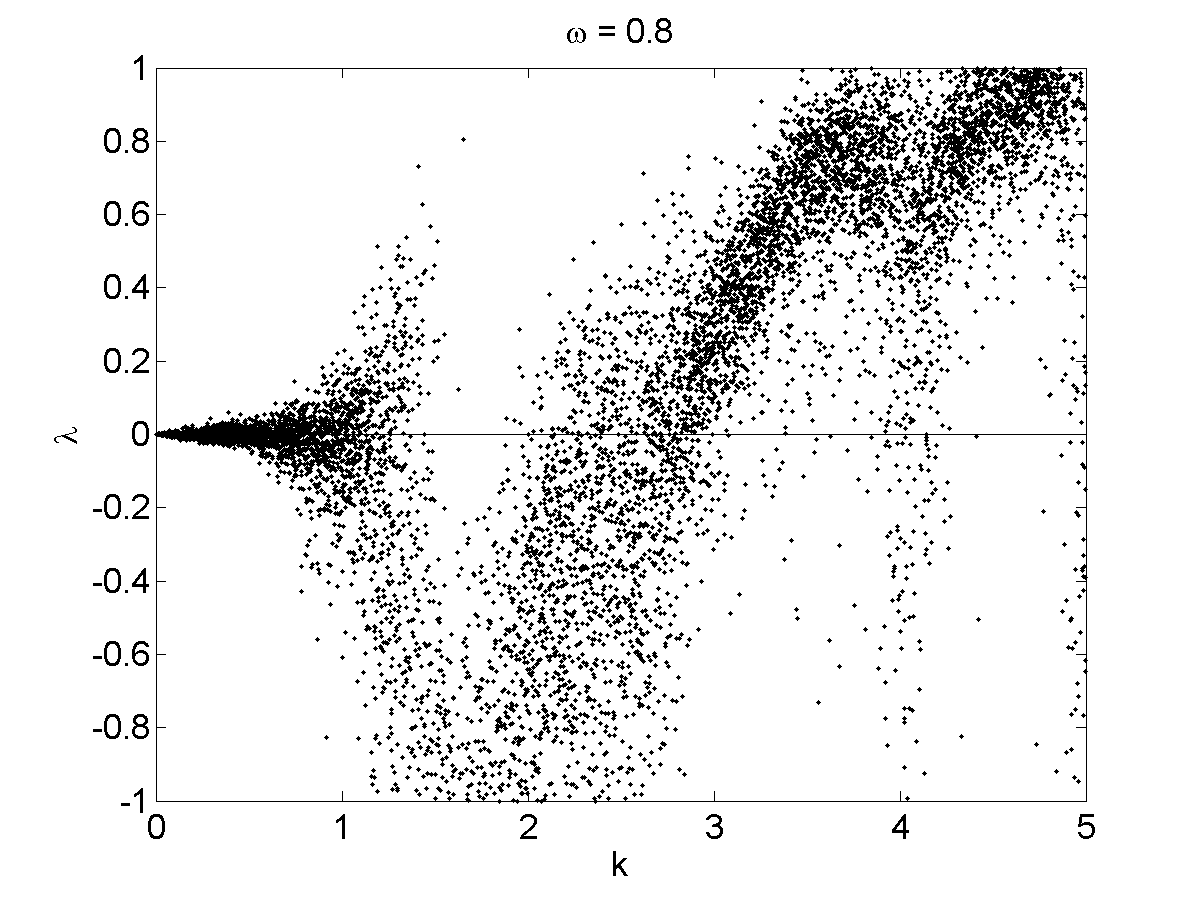
\includegraphics[width=.5\textwidth]{figs/rcirc_u_lyap_10000_L_03_w_08_k.png}\\
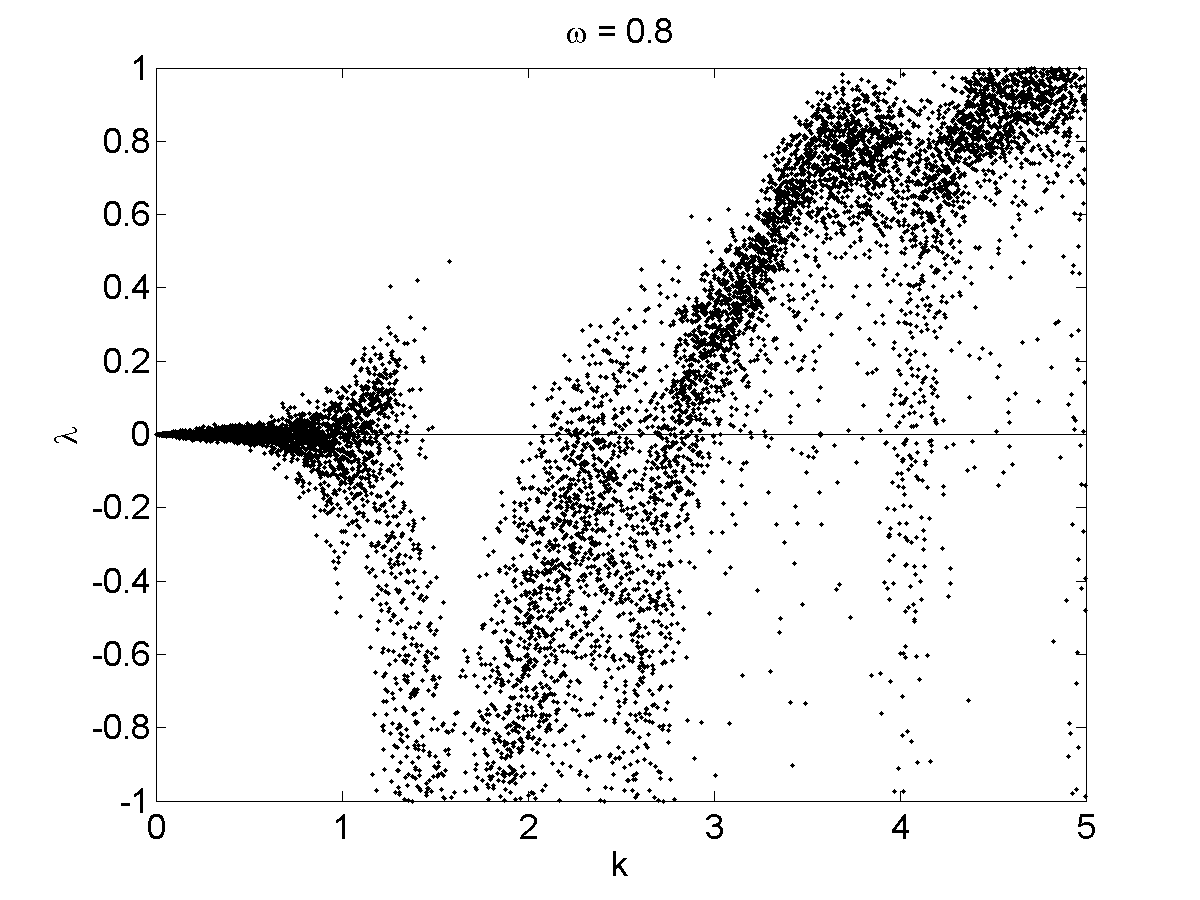
\includegraphics[width=.5\textwidth]{figs/rcirc_u_lyap_10000_L_05_w_08_k.png}\hfill
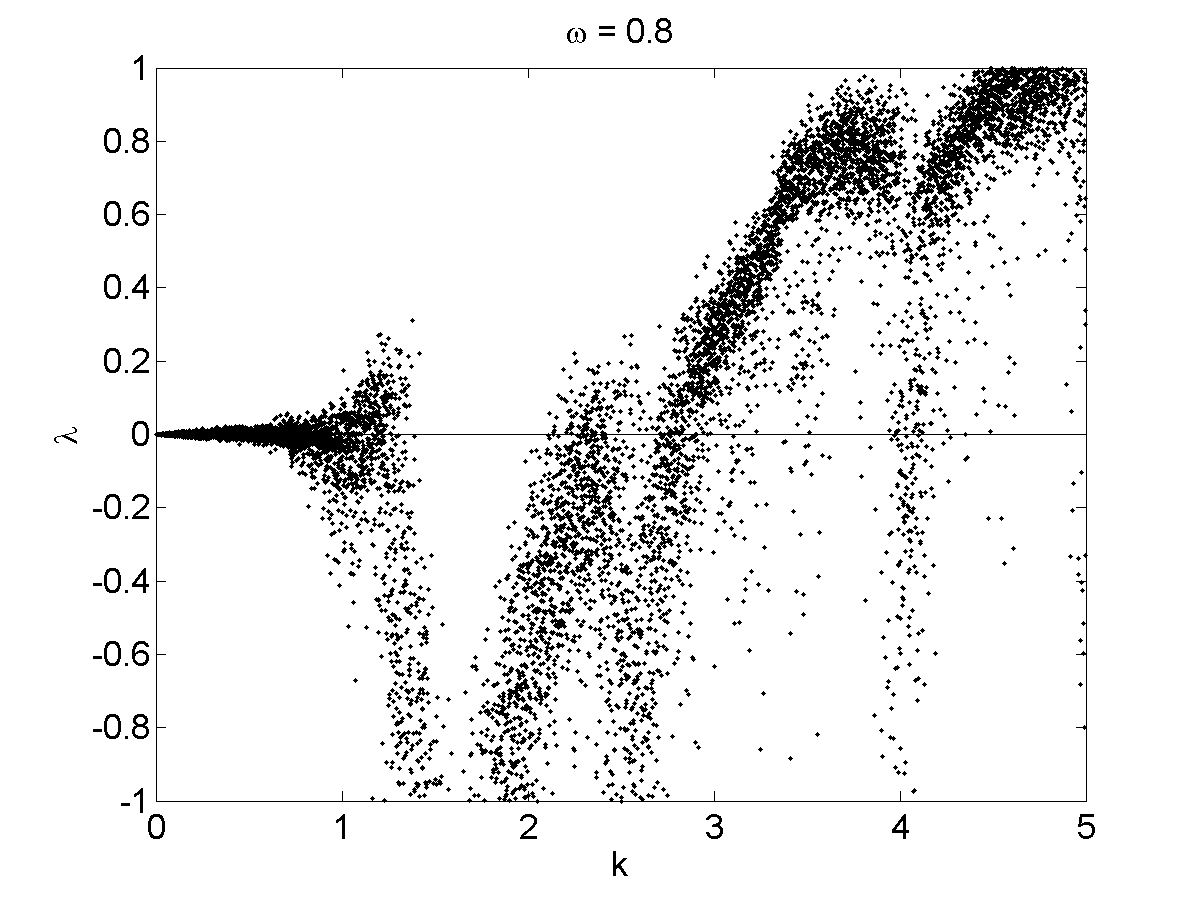
\includegraphics[width=.5\textwidth]{figs/rcirc_u_lyap_10000_L_07_w_08_k.png}\\
\end{figure}

A plot of the average number of orbits
(Figure~\ref{fig:avgcircorbs}) for the random process based on the
uniform distribution shows the largest number of orbits over 1000
simulations is period 1. The parameters tested in this simulation were
for $k=1, \omega=0.1$, which corresponds to a stable period 1 region
in the bifurcation diagram (middle left in
Figure~\ref{fig:rcirctongues_u}). This demonstrates the presence of
stable high-period orbits, where previously there were only
stable period 1 orbits in the deterministic map. Interestingly, the
semi-log plot demonstrates the distribution of periodic orbits is not
exponential, since the shape of the graph is not linear.

\begin{figure}[H]\linespread{1}
\caption[Average number of period $p$ orbits for the random circle
map, $\alpha = 10^{-5}$]{Average number of period $p$ orbits for the random circle map,
  where $L=0.1$, $\omega =0.1$, $\alpha = 10^{-5}$, $\hat{\xi}_n\sim
  Unif(-M_n,M_n)$ and $k=1$. Results from 1000 simulations of these
  parameters are plotted, using a logarithmic scale for the
  $y$-axis. The error bars indicate the standard error in calculating the mean over 1000 samples.}\label{fig:avgcircorbs}
	\begin{center}
		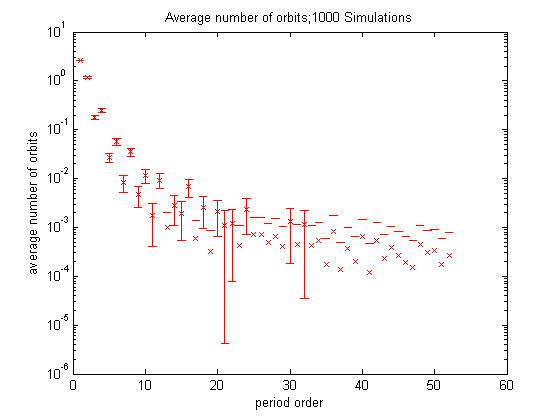
\includegraphics[scale=0.65]{figs/rcirc_avg_num_1000_sim_logscale.png}
	\end{center}
\end{figure}

% \begin{figure}[H]\linespread{1}
% \caption[Bifurcation diagram of the random
% circle map in $(x,\omega)$-space with the uniform distribution]{Bifurcation diagram of the random
% circle map for $L=0.1$, $\omega \in [0,1]$, $\Delta \omega =
% 0.001$,$\alpha = 10^{-5}$, $\hat{\xi}_n\sim Unif(-M_n,M_n)$, 
% and $k=1$. Results from 100 simulations of these parameters are
% plotted. Blue: period 1, red:
% period 2, cyan: period 3, magenta: period 4, green: period 5, black:
% period $p > 5$.} \label{fig:rcirc_bifw_u}
% 	\begin{center}
% 		\includegraphics[scale=0.65]{figs/rcirc_bif_L01_k1.png}
% 	\end{center}
% \end{figure}

Figure~\ref{fig:randdevil1_u} and Figure~\ref{fig:randdevil2_u} are
plots of the rotation number of the random circle map. Recall that a
rational rotation number $\rho = p/q$ indicates that there is a period
$q$ orbit in the map, whereas an irrational $\rho$ indicates
quasiperiodic orbits, which means chaos is a
possibility. Figure~\ref{fig:randdevil1_u} implies that decreasing $L$
introduces the most noise in the plot of rotation numbers, and
Figure~\ref{fig:randdevil2_u} shows that for $L=0.1$, there may be
chaos in the random map for values of $k<1$. In the deterministic map,
chaos appears only for $k>1$.

\begin{figure}[H]\linespread{1}
\caption[The devil's staircase for the random circle map, varying $L$
(uniform distribution), $\alpha = 10^{-5}$]{The devil's
  staircase for $L=0.05$ (left), $L=0.3$ (middle), and $L=0.5$ (right), where $k=1$,$\alpha = 10^{-5}$ and $\hat{\xi}_n\sim Unif(-M_n,M_n)$. For small $L$, the noise is more pronounced than for large $L$.}\label{fig:randdevil1_u}
\centering
\includegraphics[width=.33\textwidth]{figs/rcirc_u_devil_k1_L005.png}\hfill
\includegraphics[width=.33\textwidth]{figs/rcirc_u_devil_k1_L01.png}\hfill
\includegraphics[width=.33\textwidth]{figs/rcirc_u_devil_k1_L05.png}
\end{figure}

\begin{figure}[H]\linespread{1}
\caption[The devil's staircase for the random circle map, varying $k$
(uniform distribution), $\alpha = 10^{-5}$]{The devil's
  staircase for $k=0.7$ (left), $k=1$ (middle), and $k=1.5$
  (right). In each plot, $\alpha = 10^{-5}$,$\hat{\xi}_n\sim Unif(-M_n,M_n)$ and $L = 0.1$.}\label{fig:randdevil2_u}
\centering
\includegraphics[width=.329\textwidth]{figs/rcirc_u_devil_k07_L01.png}\hfill
\includegraphics[width=.329\textwidth]{figs/rcirc_u_devil_k1_L01.png}\hfill
\includegraphics[width=.329\textwidth]{figs/rcirc_u_devil_k15_L01.png}
\end{figure}

Figure~\ref{fig:kde1_u} is a histogram of the observed number of
rotation numbers for fixed $L=0.1,k=1,\alpha=10^{-5},\omega=0.45$. Next to the
histogram is the kernel density estimator for this distribution of
rotation numbers. Kernel density estimation is a non-parametric way of
estimating the probability density function of a random variable. This
method makes no assumptions regarding the density functions of the
observed random variables. The key parameter in kernel density
estimation is the bandwidth, which is also known as a smoothing
parameter. The smaller the bandwidth, the less smooth the density
estimate. This may exaggerate some characteristics of the sample. In
MATLAB, the default bandwidth is $h=1.5141$, and this bandwidth is reflected
in Figure~\ref{fig:kde1_u}. The kernel density estimation suggests
that for this $(L,k,\omega)$-tuple, the distribution of rotation numbers may be
normal. Using a larger $h$ would smooth the estimation so that the
curve resembles the normal density function. 

\begin{figure}[H]\linespread{1}
\caption[Histogram and kernel density estimator of rotation numbers in the random circle
map, $\alpha = 10^{-5}$]{Histogram of rotation numbers in the random circle map, where
  $L=0.1$, $k=1$, $\alpha = 10^{-5}$, $\hat{\xi}_n\sim
  Unif(-M_n,M_n)$, and $\omega = 0.45$. Results from 1000 simulations
  are plotted.}\label{fig:kde1_u}
\centering
\includegraphics[width=.5\textwidth]{figs/hist_rho_k1_L01_om045.png}\hfill
\includegraphics[width=.5\textwidth]{figs/kde_rho_k1_L01_om045.png}
\end{figure}

\subsection{Normal Distribution}
Like the uniformly distributed case, the randomized circle map for normally distributed $\hat{\xi}_n$ has a set of Arnold Tongues (Figure~\ref{fig:rcirctongues_n}) that has almost no similarity to the deterministic
case. The same trend in $L$ is observed: small $L$ values seem to correspond
with asymmetry and loss of tongue-shape, and aspects of the
deterministic map are recovered for larger $L$. 

Again, the randomness appears to have an overall destabilizing effect on the dynamics of the
map. In comparison to the uniform case, for $L=0.05$, there seem to be
more high-period orbits in the region where there is typically only
period 1 fixed points (upper left). Furthermore, the shape of the
tongues emerges more clearly for $L=0.1$ in the uniform case, and the
normal case appears more disjoint. Perhaps the difference between the
normal and uniform cases is best highlighted in the diagrams for
$L=0.3$. There are many high-period orbits for $\omega \approx 0.5$ in
the uniform case, but very few in the normal case. Also, there is a period
2 tongue on the right side of the plot in the normal case, which is
absent in the uniform case. For $L=0.9$, the uniform case exhibits period 2 and 4 orbits
for $\omega=0.5$, but the normal case only shows period 2 orbits, hinting that low-period orbits are more stable for the normal case. 

The Lyapunov exponents for a fixed $k$ and varying $\omega$
(Figure~\ref{fig:rcirclyap_n}) and exponents for fixesd $\omega$ and
varying $k$ (Figure~\ref{fig:rcirclyap2_n}) possess some similar
qualities to the uniform case. The exponents partially confirm the
idea that the noise is destabilizing as few features of the
deterministic graph are preserved. The high density of positive values
point to chaotic behavior. The skewed distribution of Lyapunov exponents on the right side of the graph from
Figure~\ref{fig:rcirclyap_u} is replicated in
Figure~\ref{fig:rcirclyap_n}. In both the uniform and normal case
(Figure~\ref{fig:rcirclyap2_u} and Figure~\ref{fig:rcirclyap2_n}), as $L$ grows larger, more features
of the deterministic plot become apparent. For instance, when
$L=0.05$, one can only make out a very general outline of the overall
shape of the Lyapunov exponents, but for $L=0.09$, there is a tighter
bound on how far the exponents stray from their deterministic configuration. 

\begin{figure}[H]\linespread{1}  
\caption[The Arnold tongues for the random circle map, normal
distribution, $\alpha = 10^{-5}$]{The Arnold
  tongues for $k\in [0,1.5]$, $\Delta k = 0.0015$, $\omega \in [0,1]$,
  $\Delta \omega = 0.001$, $\alpha = 10^{-5}$, $\hat{\xi}_n\sim
  N(0,\alpha e^{-L|n|})$ and $L_j \in
  \{0.025,0.05,0.1,0.3,0.5,0.9\}$. $\Delta k$ and $\Delta \omega$
  represent the step size in discretizing $k$ on [0,1.5] and $\omega$
  on [0,1]. Plots are ordered left to right, and top to bottom. The colorbar
to the right demonstrates the period and corresponding color.}\label{fig:rcirctongues_n}
\centering
\includegraphics[width=.5\textwidth]{figs/tongues_norm_1000_L_0025.png}\hfill
\includegraphics[width=.5\textwidth]{figs/tongues_norm_1000_L_005.png}\\
\includegraphics[width=.5\textwidth]{figs/tongues_norm_1000_L_01.png}\hfill
\includegraphics[width=.5\textwidth]{figs/tongues_norm_1000_L_03.png}\\
\includegraphics[width=.5\textwidth]{figs/tongues_norm_1000_L_05.png}\hfill
\includegraphics[width=.5\textwidth]{figs/tongues_norm_1000_L_09.png}\\
\end{figure}

\begin{figure}[!h]
\caption[Lyapunov exponent in the random circle map (normal distribution) compared to the
deterministic map, varying $\omega$, $\alpha = 10^{-5}$]{The Lyapunov exponent for the deterministic
  circle map (top left) is compared
  to the Lyapunov exponent of the random circle map for $L \in
  \{0.05,0.1,0.3,0.5,0.9\}$, where $x_0=0.7$, $k=1.5$,$\alpha =
  10^{-5}$, and $\hat{\xi}_n\sim
  N(0,\alpha e^{-L|n|})$ for $\omega \in [0,1]$. The number of exponents computed was $N_\lambda=10,000$. Plots are read left to right, and top to bottom. }\label{fig:rcirclyap_n}
\centering
\includegraphics[width=.5\textwidth]{figs/det_circ_lyap.png}\hfill
\includegraphics[width=.5\textwidth]{figs/rcirc_n_lyap_L_005_w.png}\\
\includegraphics[width=.5\textwidth]{figs/rcirc_n_lyap_L_01_w.png}\hfill
\includegraphics[width=.5\textwidth]{figs/rcirc_n_lyap_L_03_w.png}\\
\includegraphics[width=.5\textwidth]{figs/rcirc_n_lyap_L_05_w.png}\hfill
\includegraphics[width=.5\textwidth]{figs/rcirc_n_lyap_L_09_w.png}\\
\end{figure}

\begin{figure}[!h]
\caption[Lyapunov exponent in the random circle map (normal distribution) compared to the
deterministic map, varying $k$, $\alpha = 10^{-5}$]{The Lyapunov exponent for the deterministic
  circle map (top left) is compared
  to the Lyapunov exponent of the random circle map for $L \in
  \{0.05,0.1,0.3,0.5,0.7\}$, where $x_0=0.7$, $\omega=0.7$,$\alpha =
  10^{-5}$, and $\hat{\xi}_n\sim
  N(0,\alpha e^{-L|n|})$ for $k \in [0,5]$. The number of exponents computed was $N_\lambda=10,000$. Plots are read left to right, and top to bottom. }\label{fig:rcirclyap2_n}
\centering
\includegraphics[width=.5\textwidth]{figs/det_circ_lyap_k.png}\hfill
\includegraphics[width=.5\textwidth]{figs/rcirc_n_lyap_L_005_k_10000.png}\\
\includegraphics[width=.5\textwidth]{figs/rcirc_n_lyap_L_01_k_10000.png}\hfill
\includegraphics[width=.5\textwidth]{figs/rcirc_n_lyap_L_03_k_10000.png}\\
\includegraphics[width=.5\textwidth]{figs/rcirc_n_lyap_L_05_k_10000.png}\hfill
\includegraphics[width=.5\textwidth]{figs/rcirc_n_lyap_L_07_k_10000.png}\\
\end{figure}

Figure~\ref{fig:randdevil1_n} and Figure~\ref{fig:randdevil2_n} are
plots of the rotation number of the random circle map for normally
distributed Fourier mode amplitudes. The uniform case
(Figure~\ref{fig:randdevil1_u}) has a discontinuous section of $\rho$
when $\omega \approx 0.2$ and $L=0.05$, whereas the normal case shows
an almost continuous section of $\rho$. This may indicate chaotic
behavior in the uniform case. Additionally, the rotation number when
$L=0.1$ (middle of Figure~\ref{fig:randdevil1_n}) appears less noisy
than the uniform case (middle of
Figure~\ref{fig:randdevil1_u}). In line with this idea, the plots in
Figure~\ref{fig:randdevil2_n} are overall smoother than in
Figure~\ref{fig:randdevil2_n}. In all, it appears the normally
distributed Fourier mode amplitudes produce smoother plots of rotation
numbers than the uniform case.

\begin{figure}[H]\linespread{1}
\caption[The devil's staircase for the random circle map, varying $L$
(normal distribution), $\alpha = 10^{-5}$]{The devil's
  staircase for $L=0.05$ (left), $L=0.3$ (middle), and $L=0.5$ (right), where $k=1$,$\alpha = 10^{-5}$ and $\hat{\xi}_n\sim N(0,\alpha e^{-L|n|})$. For small $L$, the noise is more pronounced than for large $L$.}\label{fig:randdevil1_n}
\centering
\includegraphics[width=.33\textwidth]{figs/rcirc_n_devil_k1_L005.png}\hfill
\includegraphics[width=.33\textwidth]{figs/rcirc_n_devil_k1_L03.png}\hfill
\includegraphics[width=.33\textwidth]{figs/rcirc_n_devil_k1_L05.png}
\end{figure}

\begin{figure}[H]\linespread{1}
\caption[The devil's staircase for the random circle map, varying $k$
(normal distribution), $\alpha = 10^{-5}$]{The devil's
  staircase for $k=0.7$ (left), $k=1$ (middle), and $k=1.5$
  (right). In each plot, $\alpha = 10^{-5}$,$\hat{\xi}_n\sim
  N(0,\alpha e^{-L|n|})$ and $L = 0.1$. The discontinuities increase as
$k$ grows.}\label{fig:randdevil2_n}
\centering
\includegraphics[width=.33\textwidth]{figs/rcirc_n_devil_k07_L01.png}\hfill
\includegraphics[width=.33\textwidth]{figs/rcirc_n_devil_k1_L01.png}\hfill
\includegraphics[width=.33\textwidth]{figs/rcirc_n_devil_k15_L01.png}
\end{figure}

